% =============================================================================
% legoESM Scientific Guide
% Modeled after the NCAR CAM5 Scientific Guide
% =============================================================================
\documentclass[11pt,twoside]{report}

\usepackage[margin=1in]{geometry}
\usepackage{amsmath,amssymb,bm,mathtools}
\usepackage[colorlinks=true,linkcolor=blue!60!black,citecolor=green!50!black,urlcolor=blue!70!black]{hyperref}
\usepackage{booktabs}
\usepackage{enumitem}
\usepackage{titlesec}
\usepackage{graphicx}
\usepackage{fancyhdr}
\usepackage{xcolor}
\usepackage{longtable}
\usepackage{caption}
\usepackage{natbib}
\usepackage{multirow}
\usepackage{tabularx}

% --- Page style ---
\pagestyle{fancy}
\fancyhead[LE]{\small\thepage\quad\textit{legoESM Scientific Guide}}
\fancyhead[RO]{\small\textit{\leftmark}\quad\thepage}
\fancyhead[RE,LO]{}
\fancyfoot{}
\renewcommand{\headrulewidth}{0.4pt}

% --- Chapter/section formatting ---
\titleformat{\chapter}[display]
  {\normalfont\huge\bfseries}{\chaptertitlename\ \thechapter}{20pt}{\Huge}
\titleformat{\section}{\Large\bfseries}{\thesection}{1em}{}
\titleformat{\subsection}{\large\bfseries}{\thesubsection}{1em}{}
\titleformat{\subsubsection}{\normalsize\bfseries}{\thesubsubsection}{1em}{}

% --- Math shortcuts ---
\newcommand{\dd}{\mathrm{d}}
\newcommand{\pp}{\partial}
\newcommand{\half}{\tfrac{1}{2}}
\newcommand{\Rd}{R_d}
\newcommand{\cpd}{c_p}
\newcommand{\cvd}{c_v}
\newcommand{\Lv}{L_v}
\newcommand{\Ls}{L_s}
\newcommand{\Lf}{L_f}
\newcommand{\Rv}{R_v}
\newcommand{\pref}{p_0}
\newcommand{\SB}{\sigma_{\mathrm{SB}}}
\newcommand{\vect}[1]{\bm{#1}}
\newcommand{\grad}{\nabla}
\newcommand{\divg}{\nabla\!\cdot\!}
\newcommand{\curl}{\nabla\!\times\!}
\DeclareMathOperator{\sgn}{sgn}
\DeclareMathOperator{\diag}{diag}
\DeclareMathOperator{\Var}{Var}
\newcommand{\Ro}{\mathrm{Ro}}

% =============================================================================
% Document version tracks the package MAJOR.MINOR (single-sourced in the root
% pyproject.toml [project].version; see the README "Versioning" section).
\newcommand{\legoesmversion}{0.1}
\title{
  \vspace{-1cm}
  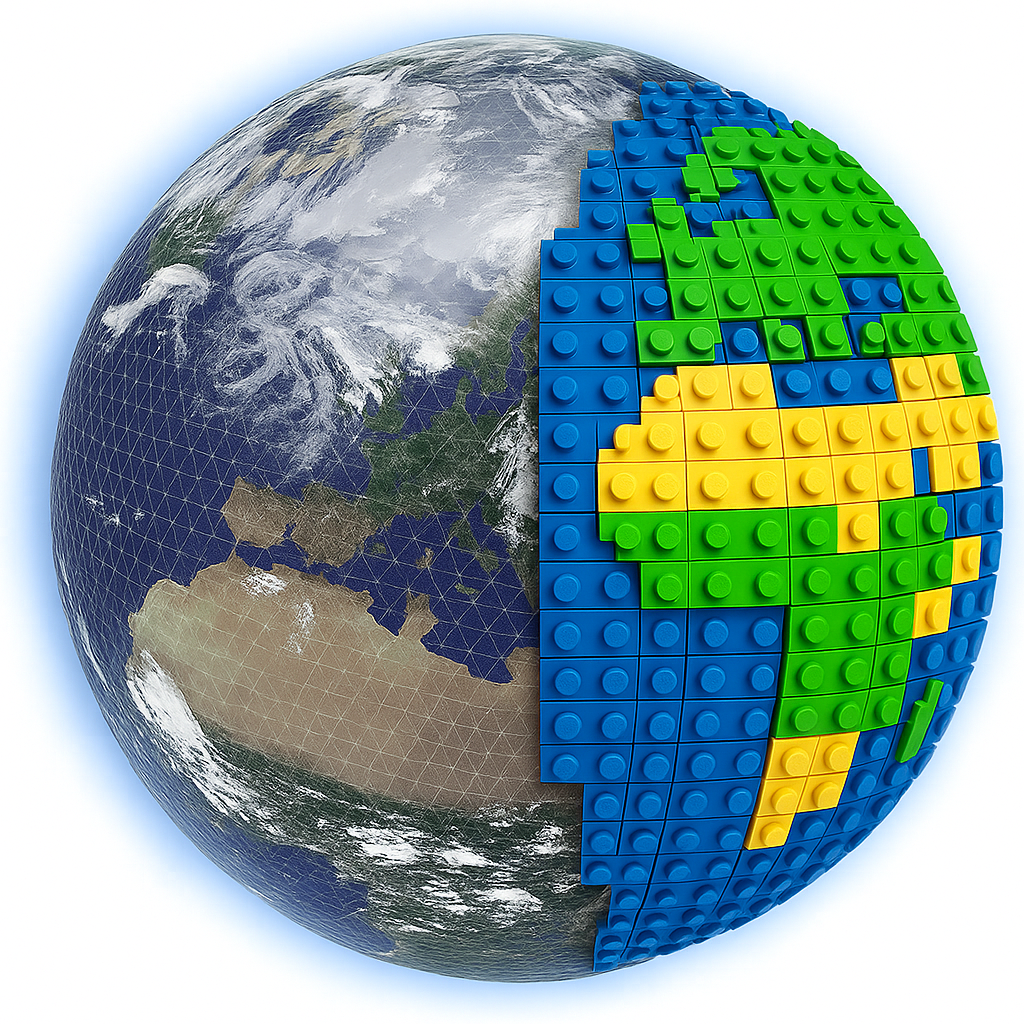
\includegraphics[width=0.35\textwidth]{../assets/legoESM.png}\\[12pt]
  \textbf{legoESM Scientific Guide}\\[6pt]
  {\Large A Fully Differentiable Earth System Model in JAX}\\[6pt]
  {\large Version \legoesmversion{} --- June 2026}
}
\author{legoESM Development Team}
\date{}

\begin{document}
\maketitle
\thispagestyle{empty}

\vfill
\noindent\textit{This document provides a comprehensive scientific description of the
legoESM Earth System Model, including governing equations, numerical methods,
and parameterisation schemes for all model components.  The structure follows
the NCAR CAM Scientific Guide convention of self-contained chapters for
dynamics, physics, ocean, land, and sea ice.}

\newpage
\tableofcontents
\newpage

% #############################################################################
\chapter{Introduction}
\label{ch:intro}
% #############################################################################

\section{Overview}

legoESM is a modular, fully differentiable Earth System Model (ESM) written
entirely in JAX.  Every component---atmosphere, ocean, land, sea ice, lake,
and biogeochemistry---is compatible with JAX's automatic differentiation
(\texttt{jit}, \texttt{grad}, \texttt{vmap}, \texttt{scan}), enabling novel
applications in data assimilation (4D-Var with exact adjoints), parameter
estimation, hybrid AI--physics modelling, and sensitivity analysis.

The model features:
\begin{itemize}[nosep]
  \item \textbf{25+ dynamical cores} spanning five discretisation families
    (C-D grid FV3, spectral, finite-volume lat-lon, C-grid lat-lon, and
    MPAS/Voronoi), with shallow water, hydrostatic primitive equation,
    and non-hydrostatic compressible Euler equation sets;
  \item \textbf{35+ physics parameterisations} for radiation, convection,
    microphysics, boundary-layer turbulence, clouds, gravity wave drag,
    and surface exchange;
  \item A \textbf{3D Boussinesq ocean} with split-explicit barotropic
    solver, KPP vertical mixing, GM-Redi eddy parameterisation, and
    biogeochemistry (abiotic carbon cycle + NPZD ecosystem);
  \item A \textbf{multi-layer land model} with Richards-equation
    soil hydrology, Johansen thermal diffusion, Farquhar--Ball-Berry
    photosynthesis, and a DALEC-990 carbon cycle;
  \item \textbf{Sea-ice dynamics} with EVP rheology, multi-category
    thickness distribution, and thermodynamic coupling;
  \item A \textbf{tile-based coupler} with Monin-Obukhov surface layer,
    area-weighted flux blending, and radiation sub-cycling;
  \item \textbf{CMIP6-class infrastructure}: CF/CMOR output, six
    experiment templates, checkpointing with SHA-256 reproducibility
    verification, and a 16-parameter tuning registry;
  \item A \textbf{Spherical Fourier Neural Operator} (SFNO) for
    learned dynamics and physics emulation.
\end{itemize}

\section{Design Principles}

\begin{enumerate}[nosep]
  \item \textbf{JAX-first}: All code uses pure-functional JAX with no
    Python loops in hot paths.  Conditional branching uses
    \texttt{jnp.where} or \texttt{jax.lax.cond} to preserve
    differentiability.
  \item \textbf{Grid-agnostic physics}: Operators implement a shared
    protocol (\texttt{GridProtocol}); physics schemes accept any grid
    via column adapters that reshape to \texttt{(ncol, nlev)}.
  \item \textbf{Modular composition}: Each parameterisation follows a
    factory pattern returning a callable
    $\texttt{physics\_fn}(\text{state}, \text{grid}, \text{coord})
    \to \text{Tendencies}$.
  \item \textbf{Unified C-D grid}: Atmosphere and ocean share the same
    FV3-style C-D grid operator module on the cubed sphere, eliminating
    code duplication and the Hollingsworth--Kallberg instability.
  \item \textbf{Pytree registration}: \texttt{Field} and state objects
    are registered as JAX pytrees for seamless autodiff through the
    entire model.
\end{enumerate}

\section{Notation and Conventions}

Throughout this document:
\begin{itemize}[nosep]
  \item Vectors are denoted in bold: $\vect{v}=(u,v)$;
  \item $\hat{f}$ denotes spectral (spherical harmonic) coefficients;
  \item Subscript $k$ indexes vertical levels (increasing downward);
  \item Half-integer subscripts ($k\pm\half$) denote layer interfaces;
  \item SI units are used unless otherwise noted;
  \item $f = 2\Omega\sin\phi$ is the Coriolis parameter.
\end{itemize}


% #############################################################################
\chapter{Software Architecture and Package Federation}
\label{ch:architecture}
% #############################################################################

The scientific content of the following chapters maps onto a concrete software
structure: legoESM is a \emph{federation} of independently-installable Python
packages that all share one import namespace.  This chapter documents that
structure --- one subsection (``subchapter'') per package --- so the equations
of later chapters can be located in code.

\section{Design: one namespace, independently-installable members}
\label{sec:arch-federation}

legoESM is a \texttt{uv} workspace of eight distribution packages laid out under
\texttt{packages/<member>/legoesm/<subpkg>/}.  All members ship into a single
\texttt{legoesm} PEP-420 \emph{namespace package}, so user code always writes
\texttt{import legoesm.<subpkg>} regardless of which wheel provides it.  The
design goal is that each Earth-system component can be installed and run on its
own---\texttt{pip install legoesm-ocean} yields a working ocean model---while a
single meta-package \texttt{legoesm} pulls the whole stack.

The members obey a strict one-way \textbf{dependency DAG}, enforced in CI by
\texttt{import-linter} contracts (\texttt{lint-imports}):
\[
  \underbrace{\texttt{core}}_{\text{substrate}}
  \;\prec\;
  \underbrace{\{\texttt{atmosphere},\,\texttt{ocean},\,\texttt{land},\,\texttt{ice}\}}_{\text{components}}
  \;\prec\;
  \underbrace{\{\texttt{coupler},\,\texttt{ml},\,\texttt{tools}\}}_{\text{orchestration}}.
\]
Components depend \emph{only} on \texttt{legoesm-core} and never on one another
or on the coupler; shared physics (e.g.\ the FV3 shallow-water barotropic
solver reused by the ocean) is exposed through the substrate or via
\texttt{importlib.metadata} entry points (\texttt{legoesm.sw\_barotropics}), not
direct cross-component imports.

\section{The substrate: \texttt{legoesm-core}}
\label{sec:arch-core}

\texttt{legoesm-core} ships the subpackages \texttt{core} (fields, operators,
state, conservation accumulators, EOS), \texttt{grids} (cubed-sphere, lat-lon,
Gaussian/spectral, MPAS/Voronoi, vertical coordinates, and the grid+complexity
\emph{capability matrix}; Chapter~\ref{ch:grids}), \texttt{runtime}
(device/precision/backend bootstrap), \texttt{parallel} (halo exchange and
reductions; Chapter on parallelism), \texttt{io}, \texttt{timestepping}
(RK integrators), and \texttt{components} (the complexity-ladder taxonomy and
component protocols), together with the loose modules \texttt{constants},
\texttt{thermo}, \texttt{registry}, and \texttt{surface\_albedo}.  It imports
nothing above itself.

\section{Earth-system components}
\label{sec:arch-components}

\subsection{\texttt{legoesm-atmosphere}}
The \texttt{atmosphere} subpackage: all atmospheric dynamical cores
(Chapter~\ref{ch:dynamics})---cubed-sphere C-D grid, spectral, lat-lon
finite-volume and C-grid, MPAS/Voronoi, and SFNO---the physics parameterisation
packages (radiation, convection, microphysics, boundary layer, clouds,
gravity-wave drag), and the dycore-free single-column model (SCM).

\subsection{\texttt{legoesm-ocean}}
The \texttt{ocean} subpackage: the 3-D split-explicit Boussinesq ocean
(baroclinic/barotropic on cubed-sphere, lat-lon C-grid, and MPAS), vertical and
lateral mixing (KPP, GM-Redi, tidal), bottom drag and surface forcing,
biogeochemistry, the idealized-experiment suite, the centennial spin-up library,
and the peer-comparison fidelity harness.

\subsection{\texttt{legoesm-land}}
The \texttt{land} subpackage: slab (bucket-hydrology) and multi-layer
(Richards-equation, Johansen-thermal) land, the DALEC carbon cycle, snow, and
PFT-weighted parameter providers.

\subsection{\texttt{legoesm-ice}}
The \texttt{ice} subpackage: thermodynamic slab and EVP/mEVP dynamic sea ice
with the multi-category ice-thickness distribution and optional snow/brine/
ridging/pond physics.

\section{Orchestration: coupler, ML, and tools}
\label{sec:arch-orchestration}

\subsection{\texttt{legoesm-coupler}}
The \texttt{coupler} subpackage (tile-based surface coupling, bulk-flux and
surface-energy closure; Chapter~\ref{ch:coupling}) and the \texttt{driver}
subpackage (\texttt{ModelDriver} for atmosphere-only AMIP, \texttt{CoupledESMDriver}
for full coupling, \texttt{EarthSystemDriver} for arbitrary compositions, plus
the reproducibility \emph{run manifest}).

\subsection{\texttt{legoesm-ml}}
The \texttt{ml} (SFNO blocks, spectral convolutions, conservation-aware losses),
\texttt{training} (differentiable training driver, ERA5 ingestion, S2S
workflows), and \texttt{da} (variational 4D-Var on \texttt{jax.grad} through the
compiled segment kernel) subpackages.

\subsection{\texttt{legoesm-tools}}
The \texttt{forcing} (GHG/ozone/aerosol/SST/runoff loaders), \texttt{diagnostics}
(energy/mass budgets, column integrals, and the conservation PASS/FAIL
\emph{gates}), \texttt{experiments} (including the shared component-agnostic
\emph{test-matrix framework}, \texttt{experiments.matrix}), and
\texttt{visualization} subpackages.

\section{Reproducibility, scripts, and experiments}
\label{sec:arch-reproducibility}

Runnable code lives in bucketed directories under \texttt{scripts/}:
\texttt{run/} (production drivers), \texttt{matrix/} (the complexity-tiered
test-matrix runners), \texttt{experiment/} (the template/provenance harness:
\texttt{init\_experiment}, \texttt{validate\_templates}, \texttt{fetch\_data},
\texttt{lego\_detect\_machine}), and \texttt{bench/}, \texttt{plot/},
\texttt{validate/}, \texttt{data/}.  Experiments are versioned, tier-annotated
YAML \emph{templates} (\texttt{config/templates/}) resolved into a runnable
directory; every run writes a \texttt{run\_manifest.json} (resolved config,
state digest, git commit, and library versions) so that
\texttt{legoesm reproduce} can re-execute it bit-for-bit.  Tests carry
complexity-tier markers \texttt{tier0}--\texttt{tier3} (research $\to$
operational) and assert conservation through the same gates as the matrix
runners.


% #############################################################################
\chapter{Grid Systems and Coordinates}
\label{ch:grids}
% #############################################################################

\section{Cubed-Sphere Grid}
\label{sec:cubed-sphere}

Six faces of a cube are mapped to the sphere via \textbf{gnomonic (central)
projection}.  Let $(\alpha_x,\alpha_y)\in[-\pi/4,\pi/4]^2$ be gnomonic
coordinates on a face.

\subsection{Face-to-Cartesian Mapping}

For face~0 ($+x$ face):
\begin{equation}
  (x,y,z) = \bigl(1,\;\tan\alpha_x,\;\tan\alpha_y\bigr).
\end{equation}
Points are normalised to the unit sphere: $\hat{\vect{r}}=\vect{r}/|\vect{r}|$,
with geographic coordinates $\lambda=\mathrm{atan2}(\hat y,\hat x)$,
$\phi=\arcsin(\hat z)$.

\subsection{Cell Area}
\begin{equation}
  \Delta A = \frac{R^2\,\Delta\alpha^2}
    {\cos^2\!\alpha_x\,\cos^2\!\alpha_y\,D^3},
  \qquad D = \sqrt{1+\tan^2\!\alpha_x+\tan^2\!\alpha_y},
  \qquad \Delta\alpha=\frac{\pi}{2n}.
\end{equation}

\subsection{Grid Spacing}

Great-circle distances use the chord-to-arc formula:
\begin{equation}
  d = R\cdot 2\arcsin\!\Bigl(\frac{|\vect{r}_1-\vect{r}_2|}{2}\Bigr).
\end{equation}
The minimum grid spacing on a C$n$ cubed sphere is
\begin{equation}
  \Delta x_{\min} = \frac{\pi R}{2n\sqrt{3}},
\end{equation}
occurring at the cube corners where the gnomonic distortion is maximal.

\subsection{Grid Angle and Wind Rotation}

The angle $\theta$ between the grid $x$-axis and geographic east:
\begin{equation}
  \theta = \mathrm{atan2}\!\Bigl(\frac{\pp\phi}{\pp i},\;
  \frac{\pp\lambda}{\pp i}\cos\phi\Bigr).
\end{equation}
Wind rotation between geographic $(u_E,v_N)$ and grid-aligned $(u_g,v_g)$:
\begin{equation}
  \begin{pmatrix}u_E\\v_N\end{pmatrix}
  =\begin{pmatrix}\cos\theta&-\sin\theta\\\sin\theta&\cos\theta\end{pmatrix}
  \begin{pmatrix}u_g\\v_g\end{pmatrix}.
\end{equation}

\subsection{Halo Exchange}

Scalar fields are exchanged directly across the six-face connectivity table.
Vector fields are first rotated to geographic components, padded as scalars,
then rotated back.  Two halo widths are supported: halo\,=\,1 for second-order
and MUSCL stencils, and halo\,=\,2 for PPM/WENO5 and biharmonic operators.

\paragraph{Native 4D halo exchange.}
All 3D operators use a 4D halo path (\texttt{pad\_halo\_4d},
\texttt{pad\_halo\_vector\_4d}) that exchanges all vertical levels in a
single MPI message per neighbour, replacing the earlier
\texttt{vmap(pad\_halo)} path which issued $n_{\mathrm{lev}}$ separate
messages.

\paragraph{MPI differentiability.}
All \texttt{sendrecv} calls go through a \texttt{@jax.custom\_vjp}
wrapper (\texttt{\_sendrecv\_vjp} in \texttt{halo\_exchange.py}) that
swaps source and destination ranks in the backward pass, enabling
\texttt{jax.grad} through distributed halo exchange.  Only
\texttt{allreduce(SUM)} is AD-safe among MPI reductions;
\texttt{MAX}/\texttt{MIN}/\texttt{allgather}/\texttt{bcast} are used
only in diagnostics and are not differentiable.


% ---------------------------------------------------------------------------
\section{Gaussian Grid and Spectral Transforms}
\label{sec:spectral-grid}

The spectral dynamical cores use a Gaussian grid with triangular truncation
at total wavenumber $n_{\max}$.

\subsection{Grid Dimensions}
\begin{equation}
  n_{\mathrm{lat}} = \lceil\tfrac{3}{2}(n_{\max}+1)\rceil_{\mathrm{even}},
  \qquad n_{\mathrm{lon}} = 2\,n_{\mathrm{lat}},
  \qquad n_{\mathrm{sh}} = \frac{(n_{\max}+1)(n_{\max}+2)}{2}.
\end{equation}
Latitudes are Gaussian quadrature points $\mu_k=\sin\phi_k$ with weights
$w_k$; longitudes are equispaced.

\subsection{Associated Legendre Polynomials}

Fully normalised ($4\pi$) polynomials $P_n^m(\mu)$ satisfy
$\int|Y_n^m|^2\,\dd A=1$.  Computed via the recursion:
\begin{align}
  P_m^m &= -\sqrt{\frac{2m+1}{2m}}\;\sqrt{1-\mu^2}\;P_{m-1}^{m-1},\\
  P_n^m &= \sqrt{\frac{4n^2-1}{n^2-m^2}}
    \Bigl(\mu\,P_{n-1}^m -
    \sqrt{\frac{(n-1)^2-m^2}{4(n-1)^2-1}}\;P_{n-2}^m\Bigr).
\end{align}
The derivative operator $H_n^m=-(1-\mu^2)\,\dd P_n^m/\dd\mu$ is used for
meridional gradients.

\subsection{Spherical Harmonic Transforms}

\paragraph{Analysis (grid $\to$ spectral).}
\begin{equation}
  \hat f_{nm} = 2\pi\sum_k w_k\,P_n^m(\mu_k)\,\tilde f_m(\mu_k),
  \qquad \tilde f_m = \frac{1}{n_{\mathrm{lon}}}\,\mathrm{FFT}[f]_m.
\end{equation}

\paragraph{Synthesis (spectral $\to$ grid).}
\begin{equation}
  f(\phi,\lambda) = \mathrm{iFFT}\Bigl[\sum_{n=m}^{n_{\max}}\hat f_{nm}\,P_n^m(\mu)\Bigr].
\end{equation}

\subsection{Spectral Operators}

Laplacian eigenvalue:
$\nabla^2\hat f_{nm}=-n(n+1)/a^2\cdot\hat f_{nm}$.
Inverse Laplacian:
$\nabla^{-2}\hat f_{nm}=-a^2/[n(n+1)]$ for $n>0$.
Hyperdiffusion:
$-\nu[n(n+1)/a^2]^p\,\hat f_{nm}$.

\subsection{Velocity from Vorticity and Divergence}

Streamfunction $\psi=\nabla^{-2}\zeta$, velocity potential
$\chi=\nabla^{-2}\delta$.  Velocity reconstruction:
\begin{equation}
  u\cos\phi = \frac{\pp\psi}{\pp\theta}+\frac{\pp\chi}{\pp\lambda},
  \qquad
  v\cos\phi = \frac{\pp\psi}{\pp\lambda}-\frac{\pp\chi}{\pp\theta},
\end{equation}
where $\theta$ is colatitude.


% ---------------------------------------------------------------------------
\section{Lat-Lon Grid}
\label{sec:latlon-grid}

A uniform $n_{\mathrm{lat}}\times n_{\mathrm{lon}}$ latitude-longitude grid
with A-grid (collocated) staggering.  All operators use second-order centred
differences.  A Fourier polar filter is applied to tendencies at high
latitudes to prevent the CFL constraint from becoming prohibitively small
near the poles.


% ---------------------------------------------------------------------------
\section{Voronoi/MPAS Grid}
\label{sec:voronoi-grid}

An unstructured Voronoi tessellation generated from an icosahedral parent
mesh.  The TRiSK (Thuburn--Ringler--Skamarock--Klemp) scheme provides
mimetic discrete operators on this grid:
\begin{itemize}[nosep]
  \item Scalars (height, tracers, pressure) at cell centres;
  \item Normal velocity at edges;
  \item Vorticity at vertices (triangle dual).
\end{itemize}
Variable resolution is supported by mesh refinement.


% ---------------------------------------------------------------------------
\section{Vertical Coordinates}
\label{sec:vertical}

\subsection{Sigma Coordinate}
\begin{equation}
  \sigma = p\,/\,p_s, \qquad \sigma\in[\sigma_{\mathrm{top}},\;1].
\end{equation}
Half-level interfaces $\sigma_{k+1/2}$ are uniformly spaced; full levels
$\sigma_k=(\sigma_{k-1/2}+\sigma_{k+1/2})/2$.

\subsubsection{Simmons--Burridge Geopotential}

The geopotential at full level $k$ is
\begin{equation}
  \Phi_k = \Phi_s + \Rd\!\sum_{k'=k+1}^{N-1}T_{k'}\ln\frac{\sigma_{k'+1/2}}{\sigma_{k'-1/2}}
  + \alpha_k\,\Rd\,T_k,
\end{equation}
where the Simmons--Burridge coefficient is
\begin{equation}
  \alpha_k = 1 - \frac{\sigma_{k-1/2}}{\Delta\sigma_k}
  \ln\frac{\sigma_{k+1/2}}{\sigma_{k-1/2}}.
\end{equation}

\subsubsection{Sigma-Dot (Vertical Velocity)}
\begin{equation}
  \dot\sigma_{k+1/2} =
  \frac{\sigma_{k+1/2}-\sigma_{\mathrm{top}}}{1-\sigma_{\mathrm{top}}}
  \,D_{\mathrm{tot}}
  - \sum_{k'=0}^{k}\divg\vect{v}_{k'}\,\Delta\sigma_{k'},
  \qquad D_{\mathrm{tot}}=\sum_{k'=0}^{N-1}\divg\vect{v}_{k'}\,\Delta\sigma_{k'}.
\end{equation}

\subsubsection{Pressure Velocity}
\begin{equation}
  \omega \equiv \frac{\dd p}{\dd t}
  = \sigma\,\frac{\dd p_s}{\dd t} + p_s\,\dot\sigma.
\end{equation}

\subsection{Hybrid Sigma-Pressure Coordinate}

\begin{equation}
  p(k) = A(k)\,p_{\mathrm{ref}} + B(k)\,p_s,
\end{equation}
where $A(k)\to 1,\,B(k)\to 0$ at the model top (pure pressure levels)
and $A(k)\to 0,\,B(k)\to 1$ near the surface (pure sigma).
This eliminates large pressure-gradient force errors over steep topography
that afflict the pure sigma coordinate.

\subsection{Terrain-Following Height Coordinate ($z^*$)}

Used by the non-hydrostatic compressible Euler equations:
\begin{equation}
  z^* = H\,\frac{z-z_s}{H-z_s}, \qquad
  J=\frac{\pp z}{\pp z^*}=\frac{H-z_s}{H}.
\end{equation}
A 1D reference state $(\rho_0(z),\,\theta_0(z),\,\pi_0(z))$ is
pre-computed for the perturbation formulation.

\subsection{Ocean $z^*$ Coordinate}

The ocean uses a dynamic $z^*$ coordinate with free-surface elevation $\eta$:
\begin{equation}
  J(\eta) = \frac{\eta+H}{H_{\max}},
\end{equation}
where $H$ is the resting depth.


% #############################################################################
\chapter{Coupling of Dynamics and Physics}
\label{ch:coupling}
% #############################################################################

\section{Physics Pipeline}

The \texttt{PhysicsPipeline} class composes all physical parameterisations
into a single callable that is invoked once per dynamics timestep.  The
calling sequence within a single step is:

\begin{enumerate}[nosep]
  \item \textbf{Dynamics step}: Update winds, temperature, surface pressure,
    and tracers via the selected dynamical core.
  \item \textbf{Physics step}: Apply parameterisations in the following order:
    \begin{enumerate}[nosep]
      \item Radiation (with optional sub-cycling),
      \item Deep convection,
      \item Shallow convection / large-scale condensation,
      \item Cloud microphysics,
      \item Boundary-layer turbulence and vertical diffusion,
      \item Gravity wave drag,
      \item Surface fluxes (tile coupler).
    \end{enumerate}
  \item \textbf{Conservation fixers}: Mass, moisture, and optionally energy.
  \item \textbf{Diagnostics}: Energy budget, monthly means, snapshots.
\end{enumerate}

\section{Radiation Sub-Cycling}

Radiation is the most expensive physics component.  The pipeline supports
calling radiation every $N_{\mathrm{rad}}$ dynamics steps while holding
radiative heating rates constant between calls.  The branching is implemented
via \texttt{jax.lax.cond} with both branches returning identical array
shapes and dtypes.

\section{Grid-Agnostic Column Adapter}

The \texttt{ColumnAdapter} reshapes any grid's 3D state into a
\texttt{(ncol, nlev)} column format for physics, then unflattens back
to the native grid shape.  This allows all physics schemes to operate
on simple column arrays regardless of the underlying horizontal
discretisation.

\section{Time-Split vs Process-Split}

legoESM uses \textbf{time-split} coupling: dynamics and physics operate
sequentially within each timestep.  Physics tendencies are computed from
the dynamics-updated state and applied as a forward-Euler update.  This
is natural for the finite-volume dycores that use a Lagrangian vertical
coordinate internally.


% #############################################################################
\chapter{Atmospheric Dynamics}
\label{ch:dynamics}
% #############################################################################

This chapter describes the governing equations and numerical methods for each
dynamical core.  Cores are organised by equation system (shallow water,
hydrostatic primitive equations, non-hydrostatic compressible Euler),
then by discretisation.

% ---------------------------------------------------------------------------
\section{Shallow Water Equations}
\label{sec:sw}

The rotating shallow water equations in \textbf{vector-invariant form}:
\begin{align}
  \frac{\pp h}{\pp t} &= -\divg(h\,\vect{v}),
  \label{eq:sw-mass}\\
  \frac{\pp u}{\pp t} &= (\zeta+f)\,v - \frac{\pp B}{\pp x} + D_u,
  \label{eq:sw-u}\\
  \frac{\pp v}{\pp t} &= -(\zeta+f)\,u - \frac{\pp B}{\pp y} + D_v,
  \label{eq:sw-v}
\end{align}
where $B=\half(u^2+v^2)+g(h+h_s)$ is the Bernoulli function,
$\zeta=\pp v/\pp x - \pp u/\pp y$ is the relative vorticity,
and $D_u,D_v$ represent hyperdiffusion.

\subsection{C-D Grid Cubed-Sphere Discretisation}

This is the primary shallow water solver, using the FV3-style C-D grid
staggering of \citet{Lin2004} and \citet{PutmanLin2007}.

\paragraph{Prognostic variables.}
D-grid winds $(u_d,v_d)$ at cell corners, shape $(6,n\!+\!1,n\!+\!1)$;
height $h$ at cell centres, shape $(6,n,n)$.

\paragraph{D-grid vorticity.}
Vorticity at each cell corner is the discrete circulation divided by the
corner dual-cell area:
\begin{equation}
  \zeta_{\mathrm{corner}} = \frac{1}{A_c}\oint\vect{u}\cdot\dd\vect{l}
  \approx \frac{1}{A_c}\bigl[u^D_{i,j}\Delta x - u^D_{i+1,j}\Delta x
  + v^D_{i,j+1}\Delta y - v^D_{i,j}\Delta y\bigr].
\end{equation}
This circulation-based discretisation is exact on the D-grid and
\textbf{eliminates the Hollingsworth--Kallberg instability} that plagues
A-grid vorticity operators.

\paragraph{Arakawa--Lamb gradient.}
The Bernoulli gradient at D-grid corners uses a 4-point average:
\begin{equation}
  \left.\frac{\pp B}{\pp x}\right|_{i+\half,j+\half}
  = \frac{B_{i+1,j}+B_{i+1,j+1}-B_{i,j}-B_{i,j+1}}{2\Delta x}.
\end{equation}

\paragraph{C-grid mass flux.}
C-grid velocities are diagnosed from D-grid winds by face-edge averaging.
Scalar transport uses upwind C-grid mass fluxes:
\begin{equation}
  \frac{\dd h}{\dd t} = -\frac{1}{A}
  \bigl[(hu_c)_{i+\half,j}-(hu_c)_{i-\half,j}
  +(hv_c)_{i,j+\half}-(hv_c)_{i,j-\half}\bigr].
\end{equation}

\paragraph{FV3-faithful PPM transport (v3.9).}
As of v3.9, the C-D grid operator module underwent a complete rewrite
to implement FV3-faithful Piecewise Parabolic Method (PPM) transport
\citep{ColellaWoodward1984} on staggered D/C grids.  Key elements include:
\begin{itemize}[nosep]
  \item PPM reconstruction with Colella--Woodward monotonicity limiters
    for all scalar fields;
  \item Flux-form mass transport on staggered D-grid and C-grid;
  \item Corrected geographic-to-grid wind rotation eliminating
    sign errors in cross-face interpolation;
  \item Tuned hyperdiffusion with physical $e$-folding time
    ($\nu_4 = \Delta x^4/\tau_{\mathrm{efold}}$).
\end{itemize}
The module spans approximately 740~lines of JAX code.

\paragraph{FV3 forward--backward shallow-water core (v4.0).}
An FV3-exact implementation of the complete c\_sw/d\_sw forward--backward
stepping algorithm is provided in \texttt{fv3\_sw\_core.py}.  The forward
step (c\_sw) computes C-grid mass fluxes and height tendencies; the backward
step (d\_sw) updates D-grid winds using the vorticity flux and Bernoulli
gradient.

\subparagraph{d2a2c\_vect.}
The D-grid $\to$ A-grid $\to$ C-grid vector conversion faithfully ports
the GFDL FV3 algorithm, including:
\begin{itemize}[nosep]
  \item Edge-boundary stencils with one-sided 4-point interpolation at
    cube-face edges;
  \item Non-orthogonality corrections via $\cos\alpha$ and
    $(\sin^2\!\alpha)^{-1}$ corner metrics;
  \item Halo-aware padding with face-boundary detection.
\end{itemize}

\subparagraph{PPM wind and vorticity transport.}
C-grid wind tendencies (\texttt{xtp\_u}, \texttt{ytp\_v}) and absolute
vorticity flux use Piecewise Parabolic Method reconstruction with
FV3-specific interpolation coefficients ($A_1$, $A_2$, $C_1$--$C_3$)
and Colella--Woodward monotonicity limiters.

\subparagraph{Cell-centred kinetic energy.}
Kinetic energy is computed from A-grid velocities at cell centres, with
an optional 4th-order averaging stencil (\texttt{a2b\_ord4}).

\paragraph{Duo-grid sub-grid metrics (Mouallem et al.\ 2023).}
The cubed-sphere C-D grid computes 9-point sub-grid angle metrics per cell:
\begin{equation}
  \sin\alpha_{\mathrm{sg}},\;\cos\alpha_{\mathrm{sg}} \in \mathbb{R}^{6 \times n \times n \times 9},
\end{equation}
encoding the local deviation from orthogonality at cell centres, edge
midpoints, and corners.  These enable FV3-faithful flux scaling at
cube-face boundaries where the gnomonic projection introduces
non-orthogonality.  Additional C-D grid metrics:
\begin{itemize}[nosep]
  \item Centre-to-centre distances $\Delta x_c$ (shape $6 \times (n\!+\!1) \times n$)
    and $\Delta y_c$ (shape $6 \times n \times (n\!+\!1)$);
  \item Non-orthogonality factors $\cos\alpha_{\mathrm{corner}}$ and
    $(\sin^2\!\alpha_{\mathrm{corner}})^{-1}$ at D-grid corners.
\end{itemize}

\paragraph{Fidelity calibration and 3D edge-artifact sentinels.}
The C-D-grid FV3 port is gated on a dual-target Williamson 2 / Williamson 5
calibration: at C36 with $\Delta t=300$~s the production knobs
\texttt{div\_damp\_order = 8} and \texttt{damp\_v = 0.030} (iter-1030)
satisfy both criteria simultaneously --- Williamson 2 v-wind error
$|v_{\mathrm{ll}}|<0.119$~m\,s$^{-1}$ and Williamson 5 day-5 height
$h>0$ with $|\vect{u}|<80$~m\,s$^{-1}$.  A 48-test sentinel suite
exercises the full 3D coverage matrix
(hydrostatic / non-hydrostatic $\times$ rest / edge / long
integration $\times$ cube-edge $i,j\in\{0,n{-}1\}$) and a long
100-step cosine-bell closure within $\pm 5\%$.  Visual verification
of $v$-wind snapshots is mandatory --- error norms can improve while
edge artifacts shift in character; see \texttt{docs/fv3\_fortran\_fidelity\_review.md}
and \texttt{docs/cubed\_sphere\_edge\_artifacts.md} for the iter-1045
status snapshot.

\subsection{Lat-Lon Finite Volume Discretisation}

A-grid staggering on a uniform $n_{\mathrm{lat}}\times n_{\mathrm{lon}}$
grid.  Centred differences for all operators.  A Fourier polar filter
damps meridional wavelengths near the poles to maintain CFL stability.

\subsection{C-Grid Lat-Lon Discretisation}

Height at cell centres; $u$ at longitude interfaces; $v$ at latitude
interfaces.  Advantages: exact pressure gradient (just cell differences),
mass flux naturally at cell interfaces (no interpolation), and better
gravity wave dispersion.  The Coriolis term requires 4-point interpolation.

\subsection{TRiSK Discretisation on Voronoi Mesh}

Following \citet{Ringler2010}, the discrete operators on the Voronoi
mesh are:
\begin{align}
  \text{Divergence at cell } c: &\quad
    (\divg\vect{u})_c = \frac{1}{A_c}\sum_e n_{e,c}\,u_e\,l_e, \\
  \text{Gradient at edge } e: &\quad
    (\grad\phi)_e = \frac{\phi_{c_2}-\phi_{c_1}}{d_e}, \\
  \text{Curl at vertex } v: &\quad
    (\curl\vect{u})_v = \frac{1}{A_v}\sum_e t_{e,v}\,u_e\,d_e,
\end{align}
where $n_{e,c}$ and $t_{e,v}$ are orientation signs, $l_e$ is edge length,
$d_e$ is distance between adjacent cell centres, and $A_c,A_v$ are
cell/vertex areas.

\subsection{Spectral Shallow Water}

Vorticity--divergence formulation on the Gaussian grid:
\begin{align}
  \frac{\pp\hat\zeta}{\pp t} &= -\widehat{\divg[(\zeta+f)\vect{v}]}, \\
  \frac{\pp\hat\delta}{\pp t} &= \widehat{\curl[(\zeta+f)\vect{v}]}
    - \nabla^2\widehat{(E+\Phi+\Phi_s)}, \\
  \frac{\pp\hat\Phi}{\pp t} &= -\widehat{\divg(\Phi\,\vect{v})},
\end{align}
where $E=\half(u^2+v^2)$ and $\Phi=g\,h$.  Pseudospectral: nonlinear
products computed on the grid, then transformed to spectral space.


% ---------------------------------------------------------------------------
\section{Hydrostatic Primitive Equations}
\label{sec:pe}

Prognostic variables: $u,v$ (horizontal winds), $T$ (temperature),
$p_s$ (surface pressure), and tracers $q_i$.

\subsection{Continuous Equations}

In $\sigma$-coordinates:
\begin{align}
  \frac{\pp p_s}{\pp t} &= -\int_0^1 \divg(p_s\,\vect{v})\,\dd\sigma,
  \label{eq:pe-ps}\\
  \frac{\pp u}{\pp t} &= (\zeta+f)\,v - \frac{\pp B}{\pp x}
  - \Rd T\,\frac{\pp\ln p_s}{\pp x} + D_u,
  \label{eq:pe-u}\\
  \frac{\pp v}{\pp t} &= -(\zeta+f)\,u - \frac{\pp B}{\pp y}
  - \Rd T\,\frac{\pp\ln p_s}{\pp y} + D_v,
  \label{eq:pe-v}\\
  \frac{\pp T}{\pp t} &= -\divg(T\,\vect{v})+T\,\divg\vect{v}
  - \dot\sigma\,\frac{\pp T}{\pp\sigma}
  + \kappa\,T\,\frac{\omega}{p} + Q,
  \label{eq:pe-T}
\end{align}
where $B=K+\Phi$, $K=\half(u^2+v^2)$, and $\kappa=\Rd/\cpd$.
The adiabatic heating term $\kappa T\omega/p$ represents compression
warming during descent.

\subsection{C-D Grid Cubed-Sphere Discretisation}
\label{sec:pe-cdgrid}

Prognostic state: $u_d,v_d$ at D-grid corners $(6,n\!+\!1,n\!+\!1,N_{\mathrm{lev}})$;
$T$ and $p_s$ at cell centres.  Spatial operators are identical to the
shallow water C-D grid (Section~\ref{sec:sw}), extended to 3D with:
\begin{itemize}[nosep]
  \item Simmons--Burridge geopotential integration (Section~\ref{sec:vertical});
  \item Sigma-dot computation with discrete continuity closure;
  \item Upwind vertical advection: $-\dot\sigma\,\pp f/\pp\sigma$.
\end{itemize}

\subsection{Spectral Transform Discretisation}
\label{sec:spe}

On the Gaussian grid, the momentum equations are recast in the
vorticity--divergence form \citep{Bourke1972}:
\begin{align}
  \frac{\pp\hat\zeta}{\pp t} &=
  \widehat{\curl[(\zeta+f)\vect{v}]}
  + \widehat{\text{vert.\ adv.}} - \nu\nabla^{2p}\hat\zeta,
  \label{eq:spe-vor}\\
  \frac{\pp\hat\delta}{\pp t} &=
  \widehat{\divg[(\zeta+f)\vect{v}]}
  - \nabla^2\widehat{(K+\Phi+\Rd T\ln p_s)}
  + \widehat{\text{vert.\ adv.}} - \nu\nabla^{2p}\hat\delta,
  \label{eq:spe-div}\\
  \frac{\pp\hat T}{\pp t} &=
  \widehat{-\divg(T\vect{v})+T\divg\vect{v}}
  - \widehat{\dot\sigma\,\pp T/\pp\sigma}
  + \widehat{\kappa T\omega/p},
  \label{eq:spe-T}\\
  \frac{\pp\widehat{\ln p_s}}{\pp t} &= -\int_0^1\hat\delta\,\dd\sigma.
  \label{eq:spe-lnps}
\end{align}

\paragraph{Spectral curl and divergence.}
For flux vectors $(U,V)=(F_u\cos\phi,\,F_v\cos\phi)$:
\begin{equation}
  \widehat{\text{curl}} = \frac{im}{a}\,\mathcal{S}\bigl[V/\cos^2\!\phi\bigr]
  + \frac{1}{a}\,\mathcal{S}_\mu[U],
  \qquad
  \widehat{\text{div}} = \frac{im}{a}\,\mathcal{S}\bigl[U/\cos^2\!\phi\bigr]
  - \frac{1}{a}\,\mathcal{S}_\mu[V],
\end{equation}
where $\mathcal{S}$ and $\mathcal{S}_\mu$ denote the SH analysis with
standard and $\dd P_n^m/\dd\mu$ Legendre matrices.  The $\cos\phi$ weighting
is absorbed into the Legendre basis, making the formulation pole-safe.

\paragraph{Semi-implicit treatment of gravity waves.}
Following \citet{HoskinsSimmons1975}, the fast gravity-wave terms are
treated implicitly.  Linearising about a reference temperature $T_{\mathrm{ref}}=300$~K
yields a Helmholtz equation per spectral mode:
\begin{equation}
  \bigl[\mathbf{I} + \alpha^2\Delta t^2\,\lambda_n\,\mathbf{\Gamma}\bigr]\,
  \hat\delta^{n+1} = \hat\delta^{\mathrm{explicit}},
\end{equation}
where $\lambda_n = n(n+1)/a^2$ is the Laplacian eigenvalue and $\mathbf{\Gamma}$
is the vertical coupling matrix.  This is pre-factored (LU decomposition)
for each wavenumber $n$ at initialisation, removing the gravity-wave CFL
constraint and allowing 3--4$\times$ larger timesteps.

\paragraph{Verification (v3.9).}
A comprehensive spectral dycore test suite validates conservation
(mass, energy, enstrophy), long-integration stability under
Held--Suarez forcing, spectral convergence with increasing truncation
wavenumber, and semi-implicit scheme correctness.  See
Chapter~\ref{ch:verification} for details.

\subsection{Lat-Lon Finite-Volume Discretisation}

Identical equations to the C-D grid version, discretised on the A-grid
lat-lon mesh with centred differences.  Polar filter applied to all
tendencies.  Optional Rayleigh sponge layer above a configurable
$\sigma$ cutoff.

\subsection{MPAS/Voronoi Discretisation}

TRiSK operators (Section~\ref{sec:sw}) extended to 3D.  Uses RK4 or
SSP-RK3 time stepping with energy- or enstrophy-conserving potential
vorticity flux options.


% ---------------------------------------------------------------------------
\section{Non-Hydrostatic Compressible Euler Equations}
\label{sec:nh}

In the $z^*$ terrain-following coordinate, the prognostic variables are
perturbations from a hydrostatically balanced reference state
$(\rho_0,\theta_0,\pi_0)$:

\begin{align}
  \frac{\pp u}{\pp t} &= (\zeta+f)\,v - \frac{\pp K}{\pp x}
  - \cpd\theta\,\frac{\pp\pi'}{\pp x} + D_u - r\,u,
  \label{eq:nh-u}\\
  \frac{\pp v}{\pp t} &= -(\zeta+f)\,u - \frac{\pp K}{\pp y}
  - \cpd\theta\,\frac{\pp\pi'}{\pp y} + D_v - r\,v,
  \label{eq:nh-v}\\
  \frac{\pp w}{\pp t} &= -\frac{\cpd\theta}{J}\,\frac{\pp\pi'}{\pp z^*}
  - g\,\frac{\theta'}{\theta_0} - r\,w,
  \label{eq:nh-w}\\
  \frac{\pp\theta'}{\pp t} &= -\divg(\theta\,\vect{v}_h)
  - \frac{w}{J}\,\frac{\pp\theta}{\pp z^*} + D_\theta,
  \label{eq:nh-theta}\\
  \frac{\pp\rho'}{\pp t} &= -\frac{1}{J}
  \Bigl[\grad_h\!\cdot\!(J\rho\,\vect{v}_h)
  + \frac{\pp(\rho w)}{\pp z^*}\Bigr],
  \label{eq:nh-rho}
\end{align}
where $r(z)$ is the Rayleigh sponge coefficient and the Exner function
perturbation is
\begin{equation}
  \pi' = \pi_0\Bigl[\Bigl(1+\frac{\rho'}{\rho_0}\Bigr)\!
  \Bigl(1+\frac{\theta'}{\theta_0}\Bigr)\Bigr]^{\Rd/\cvd}-\pi_0.
\end{equation}

\subsection{Split-Explicit Time Integration}

\paragraph{Slow modes} (SSP-RK3): advection, Coriolis, horizontal pressure
gradient force, and diffusion.

\paragraph{Fast modes} (forward--backward acoustic substeps):
vertical sound/gravity waves.  Typically $N_s=6$ substeps per RK stage.

\paragraph{Forward step (vertical velocity).}
\begin{equation}
  w^{n+1} = w^n + \Delta t_s
  \Bigl[-\frac{\cpd\theta}{J}\,\frac{\pp\pi'}{\pp z^*}
  - g\,\frac{\theta'}{\theta_0}\Bigr].
\end{equation}

\paragraph{Backward step (density, potential temperature).}
\begin{equation}
  \rho'^{n+1} = \rho'^n
  - \Delta t_s\,\frac{\pp(\rho\,w^{n+1})}{\pp z^*},
  \qquad
  \theta'^{n+1} = \theta'^n
  - \Delta t_s\,\frac{w^{n+1}}{J}\,\frac{\pp\theta}{\pp z^*}.
\end{equation}

\paragraph{Acoustic off-centering.}
To damp vertically propagating acoustic/gravity wave noise
\citep{SkamarockKlemp2008}:
\begin{equation}
  \rho'^{n+1}_{\beta} = (1+\beta)\,\rho'^{n+1} - \beta\,\rho'^{n},
\end{equation}
where $\beta\ge 0$ is the off-centering parameter (default 0.1).

\subsection{Sponge Layer}
\begin{equation}
  r(z) = r_{\max}\sin^2\!\Bigl(\frac{\pi}{2}\,
  \frac{\max(0,\,z-z_{\mathrm{bot}})}{z_{\mathrm{top}}-z_{\mathrm{bot}}}\Bigr).
\end{equation}

\subsection{Turbulence Closure: CRM, LES, and DNS}
\label{sec:crm-les-dns}

The diffusion terms $D_u,\,D_v,\,D_w,\,D_\theta$ in
Eqs.~\eqref{eq:nh-u}--\eqref{eq:nh-theta} are evaluated in flux form,
$D_\phi = \rho_0^{-1}\,\partial_j\!\bigl(\rho_0\,K_\phi\,\partial_j\phi\bigr)$
over the horizontal directions $j\in\{x,y\}$ and, optionally, the vertical
$j=z^*$ (a mass-weighted leg matching the SAM \texttt{diffuse\_*}
operators).  The \emph{same} discrete operator serves a hierarchy of three
turbulence-resolving regimes that differ only in the viscosity $K_m$ and the
grid spacing $\Delta x$; the heat and scalar diffusivity is
$K_h = K_m/\mathrm{Pr}$.

\begin{description}
\item[CRM (convection-permitting), $\Delta x\sim 1$--$4$\,km.]
The Smagorinsky--Lilly eddy viscosity
\begin{equation}
  K_m = (C_s\Delta)^2\,
  \sqrt{\max\!\bigl(0,\;|S|^2 - \mathrm{Pr}\,N^2\bigr)},
  \qquad \Delta = (\Delta x\,\Delta y\,\Delta z)^{1/3},
  \label{eq:smag}
\end{equation}
with the full strain magnitude $|S|^2 = 2\,S_{ij}S_{ij}$ (all six
components, including the vertical-shear terms $S_{13},S_{23},S_{33}$),
$C_s\approx 0.19$, and the moist sub-grid stratification cutoff $N^2$ (the
SAM \texttt{dosmagor} correction) that suppresses mixing in statically
stable layers.  The energy-containing eddies are entirely sub-grid, so
Eq.~\eqref{eq:smag} parameterizes \emph{all} turbulent transport.  This is
the configuration validated against gSAM for the GATE, LBA, and RCE deep
convection cases.

\item[LES (large-eddy simulation), $\Delta x\sim 10$--$100$\,m.]
The \emph{same} closure~\eqref{eq:smag} with $C_s\approx 0.15$ and an
optional near-wall mixing-length limiter $\ell_m=\min(C_s\Delta,\,\kappa z)$.
The energy-containing eddies are now resolved and $K_m$ models only the
inertial-subrange stress.  The gSAM reference simulations of GATE and LBA
are themselves $\Delta x=100$\,m LES, so the LES mode applies the identical
closure at the identical resolution as the oracle.

\item[DNS (direct numerical simulation), $\Delta x\to$ the Kolmogorov scale.]
No turbulence model.  $K_m$ is replaced by the constant molecular kinematic
viscosity $\nu$ (with $K_h=\nu/\mathrm{Pr}$ and $\mathrm{Pr}\approx 0.71$ for
air), yielding the molecular dissipation $\nu\nabla^2\vect{u}$ directly; all
turbulent scales down to dissipation are resolved.
\end{description}

The regime is selected by the \texttt{turbulence\_closure} parameter
(\texttt{smagorinsky} / \texttt{molecular} / \texttt{none}).  Because the
three regimes share the single discrete flux-form operator, LES and DNS are
a configuration change rather than a separate code path.  The molecular
closure has been verified to reproduce the analytical viscous decay
$\partial_t\hat u = -\nu k^2\hat u$ of an isolated shear mode to within the
time-integration error.


% ---------------------------------------------------------------------------
\section{Finite-Volume Transport}
\label{sec:fv-transport}

\subsection{MUSCL Reconstruction (2nd Order)}

Piecewise-linear reconstruction with slope limiting \citep{vanLeer1979}:
\begin{equation}
  q_L = q_i + \half\,\phi_i, \qquad q_R = q_{i+1} - \half\,\phi_{i+1},
\end{equation}
with minmod or MC (monotonised central) limiters.

\subsection{PPM Reconstruction (4th Order)}

The Piecewise Parabolic Method \citep{ColellaWoodward1984} constructs a
monotone parabola in each cell.  Fourth-order edge values:
\begin{equation}
  \hat q_{i+1/2} = \frac{7}{12}(q_i+q_{i+1})
  - \frac{1}{12}(q_{i-1}+q_{i+2}).
\end{equation}
Monotonicity constraint:
$\hat q_{i+1/2} \leftarrow \mathrm{median}(\hat q_{i+1/2},\,q_i,\,q_{i+1})$.
Colella--Woodward limiting prevents new extrema in the parabolic profile.

\subsection{WENO5 Reconstruction (5th Order)}

Three sub-stencil polynomials combined with nonlinear weights adapting to
local smoothness \citep{JiangShu1996}:
\begin{equation}
  q_L = \sum_k \omega_k\,q^{(k)}, \qquad
  \omega_k = \frac{\alpha_k}{\sum_j\alpha_j}, \qquad
  \alpha_k = \frac{d_k}{(\varepsilon+\beta_k)^2},
\end{equation}
where $d_k$ are ideal weights $(1/10,\,6/10,\,3/10)$ and $\beta_k$ are
smoothness indicators.

\subsection{Rusanov Flux}
\begin{equation}
  F = \half(h_L u_L + h_R u_R) - \half\,\alpha\,(h_R-h_L),
  \qquad \alpha=\max\!\bigl(|u_L|+c_L,\;|u_R|+c_R\bigr),
\end{equation}
where $c=\sqrt{g\,h}$ is the gravity-wave speed.


% ---------------------------------------------------------------------------
\section{Time Integration}
\label{sec:timestepping}

\subsection{SSP-RK3}

The three-stage strong-stability-preserving Runge--Kutta method
\citep{ShuOsher1988}:
\begin{align}
  \vect{u}^{(1)} &= \vect{u}^n + \Delta t\,F(\vect{u}^n), \\
  \vect{u}^{(2)} &= \tfrac{3}{4}\vect{u}^n + \tfrac{1}{4}\vect{u}^{(1)}
  + \tfrac{1}{4}\Delta t\,F(\vect{u}^{(1)}), \\
  \vect{u}^{n+1} &= \tfrac{1}{3}\vect{u}^n + \tfrac{2}{3}\vect{u}^{(2)}
  + \tfrac{2}{3}\Delta t\,F(\vect{u}^{(2)}).
\end{align}
SSP-RK(4,3) and SSP-RK(5,4) variants are also available.

\subsection{Robert--Asselin--Williams (RAW) Time Filter}

The leapfrog scheme used by the semi-implicit spectral PE solver requires
a time filter to damp the computational mode.  The \citet{Williams2009}
modification:
\begin{align}
  d^n &= \frac{\gamma}{2}\bigl(X^{n-1}-2X^n+X^{n+1}\bigr), \\
  X^n_{\mathrm{filt}} &= X^n + (1-\alpha)\,d^n, \\
  X^{n+1}_{\mathrm{filt}} &= X^{n+1} + \alpha\,d^n,
\end{align}
with $\alpha=0.5$ (default).  This restores second-order accuracy while
preserving the damping of the computational mode.

\subsection{CFL Conditions and Adaptive Hyperdiffusion}

The CFL-limited timestep:
\begin{equation}
  \Delta t_{\max} = \frac{C_{\mathrm{CFL}}\,\Delta x_{\min}}
  {(u_{\max}+c_{\mathrm{gw}})\sqrt{n_{\mathrm{dim}}}},
\end{equation}
where $c_{\mathrm{gw}}=\sqrt{gH}$ is the gravity wave speed.

The maximum stable hyperdiffusion coefficient for $p$-th order:
\begin{equation}
  \nu_p = S\cdot\frac{C(p)\,\Delta x^{2p}}{\Delta t},
  \qquad
  C(2)=\tfrac{1}{2},\quad C(4)=\tfrac{1}{8},\quad C(6)=\tfrac{1}{48},
\end{equation}
where $S\in(0,1]$ is a safety factor.  The physical e-folding time for
$2\Delta x$ waves is $\tau_{\mathrm{efold}} = \Delta x^{2p}/\nu_p$.


% #############################################################################
\chapter{Atmospheric Physics}
\label{ch:physics}
% #############################################################################

% ---------------------------------------------------------------------------
\section{Thermodynamic Preliminaries}
\label{sec:thermo}

\subsection{Saturation Mixing Ratio}

Using the Tetens (August--Roche--Magnus) formula:
\begin{equation}
  e_s(T) = 611.2\exp\!\Bigl(\frac{17.67\,T_c}{T_c+243.5}\Bigr),
  \qquad q_s = \frac{\varepsilon\,e_s}{p-e_s},
  \qquad \varepsilon=\Rd/\Rv\approx 0.622,
\end{equation}
where $T_c = T - 273.15$~K.  Over ice, the Clausius--Clapeyron form is
used:
\begin{equation}
  e_{s,i}(T) = 611.2\exp\!\Bigl[\frac{\Ls}{\Rv}
  \Bigl(\frac{1}{T_{\mathrm{freeze}}}-\frac{1}{T}\Bigr)\Bigr].
\end{equation}

\subsection{Virtual Temperature}
\begin{equation}
  T_v = T\,(1 + 0.608\,q_v - q_c - q_r - q_i).
\end{equation}

\subsection{Moist Adiabatic Lapse Rate}
\begin{equation}
  \Gamma_m = \frac{\Rd T}{\cpd p}\,
  \frac{1+\Lv q_s/(\Rd T)}{1+\Lv^2 q_s/(\cpd\Rv T^2)}.
\end{equation}


% ---------------------------------------------------------------------------
\section{Radiation}
\label{sec:radiation}

\subsection{Gray Two-Stream Radiation}
\label{sec:gray-rad}

Following \citet{Frierson2006}:

\subsubsection{Longwave Optical Depth}
\begin{equation}
  \tau(\sigma,\phi) = \bigl[f_l\,\sigma+(1-f_l)\,\sigma^4\bigr]
  \bigl[\tau_e+(\tau_p-\tau_e)\sin^2\!\phi\bigr]
  + \sum_k \tau_{\mathrm{moist}}\,q_{v,k}\,\frac{\Delta p_k}{g},
\end{equation}
where the moisture optical depth per layer is
$\Delta\tau_{\mathrm{moist},k}=\tau_{\mathrm{moist}}\,q_{v,k}\,\Delta p_k/g$,
with $\tau_e=7.2$, $\tau_p=1.8$, $f_l=0.2$,
$\tau_{\mathrm{moist}}=0.0115$~m$^2$\,kg$^{-1}$.

\subsubsection{Two-Stream Longwave Fluxes}

Layer transmittance and emissivity:
\begin{equation}
  \mathcal{T}_k = e^{-D\,\Delta\tau_k},
  \qquad \varepsilon_k = 1-\mathcal{T}_k,
  \qquad D=1.66.
\end{equation}
The diffusivity factor $D\approx 5/3$ accounts for the hemispheric-mean
angular integration.

Upward sweep from surface ($F^\uparrow_{\mathrm{sfc}}=\varepsilon_s\,\SB\,T_s^4$):
\begin{equation}
  F^\uparrow_k = \mathcal{T}_k\,F^\uparrow_{k+1} + \varepsilon_k\,\SB\,T_k^4.
\end{equation}
Downward sweep from TOA ($F^\downarrow_0=0$):
\begin{equation}
  F^\downarrow_k = \mathcal{T}_k\,F^\downarrow_{k-1} + \varepsilon_k\,\SB\,T_k^4.
\end{equation}

\subsubsection{Shortwave (Beer--Lambert)}
\begin{equation}
  F^\downarrow_{\mathrm{SW}}(k) = \frac{S_0}{4}\,
  e^{-\tau_{\mathrm{SW},0}\,\sigma_k},
  \qquad
  F^\uparrow_{\mathrm{SW}}(k) = \alpha_s\,F^\downarrow_{\mathrm{SW}}(\mathrm{sfc}),
\end{equation}
with $\tau_{\mathrm{SW},0}=0.22$, $S_0=1361$~W\,m$^{-2}$, $\alpha_s=0.31$.
Only the downward beam is absorbed; reflected SW escapes to space.

\subsubsection{Heating Rate}
\begin{equation}
  \frac{\dd T}{\dd t}\bigg|_{\mathrm{rad},k}
  = \frac{g}{\cpd}\,
  \frac{F^{\uparrow}_{\mathrm{net},k+1/2}-F^{\uparrow}_{\mathrm{net},k-1/2}}
  {p_{k+1/2}-p_{k-1/2}}.
\end{equation}

\subsection{RRTMGP Correlated-$k$ Radiation}
\label{sec:rrtmgp}

The RRTMGP backend uses JAX-RRTMGP with:
\begin{itemize}[nosep]
  \item 128 LW and 112 SW $g$-points for correlated-$k$ gas absorption;
  \item Two-stream delta-Eddington radiative transfer equation;
  \item Spectral line absorption for H$_2$O, CO$_2$, CH$_4$, N$_2$O, O$_3$;
  \item Cloud optics via liquid/ice water path and effective radii lookup
    tables;
  \item Optional aerosol optical depth with prescribed single-scattering
    albedo ($\omega_0=0.93$) and asymmetry factor ($g=0.70$).
\end{itemize}

Default trace-gas concentrations: CO$_2$=415~ppmv, CH$_4$=1900~ppbv,
N$_2$O=332~ppbv.

\subsection{Solar Geometry}

The cosine of the solar zenith angle:
\begin{equation}
  \mu_0 = \sin\phi\sin\delta + \cos\phi\cos\delta\cos h,
\end{equation}
where $\delta$ is the solar declination and $h$ is the hour angle.
Daily-mean insolation and perpetual-equinox modes are also available.


% ---------------------------------------------------------------------------
\section{Deep Convection}
\label{sec:convection}

Five convection schemes are available, all fully JAX-differentiable.

\subsection{Simplified Betts--Miller (SBM) Relaxation}
\label{sec:sbm}

Following \citet{Frierson2007}:

\subsubsection{CAPE Computation}
\begin{equation}
  \mathrm{CAPE} = \Rd\sum_k
  \max\!\bigl(0,\;T_{\mathrm{parcel},k}-T_{\mathrm{env},k}\bigr)\,
  \frac{\Delta p_k}{p_k}.
\end{equation}

\subsubsection{Smooth Trigger}
\begin{equation}
  \mathcal{F} = \sigma\!\bigl(\kappa_s(\mathrm{CAPE}-\mathrm{CAPE}_c)\bigr),
  \qquad \kappa_s=0.01\;\text{(J/kg)}^{-1}.
\end{equation}

\subsubsection{Enthalpy-Conserving Relaxation}

The reference profile $T_{\mathrm{ref}}$ is adjusted so that column-integrated
moist enthalpy is conserved:
\begin{equation}
  \sum_k\bigl[\cpd(T_{\mathrm{ref},k}-T_k)
  +\Lv(q_{\mathrm{ref},k}-q_{v,k})\bigr]\,\Delta p_k = 0.
\end{equation}
Tendencies:
\begin{equation}
  \frac{\dd T}{\dd t} = \mathcal{F}\,\frac{T_{\mathrm{ref}}-T}{\tau_c},
  \qquad
  \frac{\dd q_v}{\dd t} = \mathcal{F}\,\frac{q_{\mathrm{ref}}-q_v}{\tau_c},
  \qquad \tau_c=7200\;\text{s}.
\end{equation}

\subsubsection{Precipitation}
\begin{equation}
  P = -\frac{1}{g}\sum_k \frac{\dd q_v}{\dd t}\,\Delta p_k.
\end{equation}

\subsection{Kuo Column Moisture-Excess Scheme}

Convection proportional to column-integrated moisture excess above
saturation [kg\,m$^{-2}$].  Heating and moistening are partitioned
via a parameter $\alpha_{\mathrm{heat}}$:
\begin{align}
  MC &= \int \max(q_v - q_s, 0)\,\frac{\dd p}{g}, \\
  \frac{\dd T}{\dd t} &= \mathcal{F}\,\alpha_{\mathrm{heat}}\,
  \frac{T_{\mathrm{moist}}-T}{\tau_c}, \qquad
  \frac{\dd q_v}{\dd t} = \mathcal{F}\,(1-\alpha_{\mathrm{heat}})\,
  \frac{q_{s,\mathrm{moist}}-q_v}{\tau_c},
\end{align}
with $\alpha_{\mathrm{heat}}=0.75$ and $\tau_c=3600$~s.

\subsection{Mass-Flux Convection (Arakawa--Wu Type)}

A prognostic base mass flux $M_c$ relaxes toward an equilibrium value:
\begin{equation}
  M_{\mathrm{eq}} = \sigma\!\bigl[(\mathrm{CAPE}-\mathrm{CAPE}_{\mathrm{thresh}})
  /\mathrm{scale}\bigr]\cdot M_{\mathrm{scale}},
  \qquad
  \frac{\dd M_c}{\dd t} = \frac{M_{\mathrm{eq}}-M_c}{\tau_{\mathrm{adj}}}.
\end{equation}

The mass-flux profile is sinusoidal:
$m(p) = \sin[\pi(p_{\mathrm{base}}-p)/\Delta p]$.
The entraining updraft uses exponential dilution:
\begin{equation}
  T_u(z) = e^{-\epsilon_0 z}\,T_{\mathrm{moist}}
  + (1-e^{-\epsilon_0 z})\,T_{\mathrm{env}},
\end{equation}
with entrainment rate $\epsilon_0=10^{-3}$~m$^{-1}$ and detrainment
rate $\delta_0=10^{-3}$~m$^{-1}$.

\paragraph{Precipitation.}
Precipitation is diagnosed from detrainment of updraft condensate,
integrated over the column using layer thickness $\Delta z$:
\begin{equation}
  P = \sum_k \delta_0\,M_k\,q_{\ell,k}\,\Delta z_k
  \quad [\text{kg\,m}^{-2}\,\text{s}^{-1}],
\end{equation}
where $q_{\ell,k}=\max(q_{u,k}-q_{s,k},\,0)$ is the updraft condensate
and $M_k=M_c\,m(p_k)$ is the mass flux profile [kg\,m$^{-2}$\,s$^{-1}$].
The vertical measure $\Delta z$ is used (not $\Delta p/g$) because $M$
already carries units of mass flux per unit area, so $\delta_0\,M\,q_\ell$
has units [kg\,m$^{-3}$\,s$^{-1}$] and multiplying by $\Delta z$ [m]
yields [kg\,m$^{-2}$\,s$^{-1}$].

\subsection{EDMF Convection}

Eddy-Diffusivity Mass-Flux with a prognostic updraft area fraction $a_u$:
\begin{equation}
  \frac{\dd a_u}{\dd t} = \frac{a_{u,\mathrm{eq}}-a_u}{\tau_a},
\end{equation}
combining mass-flux (updraft) and eddy-diffusivity (environmental mixing)
contributions.

\paragraph{Precipitation.}
As in the mass-flux scheme (\S\ref{sec:microphysics}), precipitation
is diagnosed from condensate detrainment using $\Delta z$:
\begin{equation}
  P = \sum_k \delta_0\,M_{u,k}\,q_{\ell,k}\,\Delta z_k
  \quad [\text{kg\,m}^{-2}\,\text{s}^{-1}],
\end{equation}
with $M_{u,k}=\rho_k\,a_u\,w_{u,k}$ and $\delta_0=2\times10^{-3}$~m$^{-1}$.

\subsection{Deep Convective Adjustment}

The simplest parameterisation: scans bottom-to-top adjusting unstable
layer pairs toward moist-adiabatic neutrality while conserving total
enthalpy.  Uses sigmoid activation for smooth, differentiable blending.


% ---------------------------------------------------------------------------
\section{Cloud Microphysics}
\label{sec:microphysics}

\subsection{Kessler Warm-Rain Scheme}

Prognostic variables: $q_c$ (cloud water), $q_r$ (rain).

\paragraph{Saturation adjustment.}
The saturation excess is converted to a tendency (rate) by dividing by the
time step $\Delta t$:
\begin{equation}
  \frac{\dd q_v}{\dd t}\bigg|_{\mathrm{sat}}
  = -\frac{\sigma(\kappa_s(q_v-q_s))\cdot(q_v-q_s)}{\Delta t},
\end{equation}
with sigmoid sharpness $\kappa_s$.  This ensures all microphysics outputs
have consistent units of kg\,kg$^{-1}$\,s$^{-1}$.

\paragraph{Autoconversion (cloud $\to$ rain).}
\begin{equation}
  \frac{\dd q_c}{\dd t}\bigg|_{\mathrm{auto}}
  = -k_{\mathrm{auto}}\,\mathrm{softplus}(q_c - q_{c,\mathrm{thresh}}),
  \qquad k_{\mathrm{auto}}=10^{-3}\;\text{s}^{-1},\quad
  q_{c,\mathrm{thresh}}=10^{-3}\;\text{kg/kg}.
\end{equation}

\paragraph{Accretion (collection of cloud by rain).}
\begin{equation}
  \frac{\dd q_c}{\dd t}\bigg|_{\mathrm{accr}}
  = -k_{\mathrm{accr}}\,q_c\,q_r^{0.875},
  \qquad k_{\mathrm{accr}}=2.2.
\end{equation}

\paragraph{Rain evaporation.}
\begin{equation}
  \frac{\dd q_r}{\dd t}\bigg|_{\mathrm{evap}}
  = k_{\mathrm{evap}}\,\frac{q_s-q_v}{q_s}\,q_r^{0.525}.
\end{equation}

\paragraph{Sedimentation.}
Fall speed: $V_t = V_0\sqrt{\rho_{\mathrm{sfc}}/\rho}$ with $V_0=5$~m/s.

\paragraph{Latent heating.}
$\dd T/\dd t = (\Lv/\cpd)\cdot(\text{condensation} - \text{evaporation})$.

\subsection{Seifert--Beheng Two-Moment Warm Rain}

Prognostic mass ($q_c,q_r$) and number concentration ($N_c,N_r$).

\paragraph{Autoconversion.}
\begin{equation}
  \frac{\dd q_c}{\dd t}\bigg|_{\mathrm{auto}}
  = -k_{\mathrm{au}}\,q_c^2\,
  \sigma\!\bigl[\kappa(x_c - x^*)\bigr],
  \qquad x_c = \frac{q_c\,\rho}{N_c},
\end{equation}
where $k_{\mathrm{au}}=600$~m$^3$/(kg\,s), $x^*=2.6\times 10^{-10}$~kg
is the separation mass, and the sigmoid onset replaces the hard threshold.

\paragraph{Self-collection and breakup.}
\begin{equation}
  \frac{\dd N_r}{\dd t}\bigg|_{\mathrm{sc}}
  = -k_{\mathrm{sc}}\,N_r\,q_r\,\rho,
  \qquad
  \frac{\dd N_r}{\dd t}\bigg|_{\mathrm{br}}
  = +k_{\mathrm{br}}\,\sigma\bigl[\kappa(D_r-D_{\mathrm{eq}})\bigr]\,
  \bigl|\frac{\dd N_r}{\dd t}\big|_{\mathrm{sc}}\bigr|.
\end{equation}

\subsection{Morrison Double-Moment (Ice + Liquid)}

Extends the warm-rain scheme with ice-phase processes:

\paragraph{Ice nucleation (Cooper 1986).}
\begin{equation}
  N_{i,\mathrm{target}} = \frac{N_{i,0}}{\rho}\,
  \exp\!\bigl[a_C(T_{\mathrm{freeze}}-T)\bigr].
\end{equation}

\paragraph{Depositional growth.}
\begin{equation}
  \frac{\dd q_i}{\dd t}\bigg|_{\mathrm{dep}}
  = k_{\mathrm{dep}}\,\mathrm{softplus}(S_i)\,\sqrt{N_i},
  \qquad S_i = \frac{q_v}{q_{s,i}}-1.
\end{equation}

\paragraph{Bergeron process (mixed-phase).}
Cloud water converts to ice in the temperature window
$T_{\mathrm{center}}-T_{\mathrm{width}} < T < T_{\mathrm{freeze}}$:
\begin{equation}
  \frac{\dd q_c}{\dd t}\bigg|_{\mathrm{Berg}}
  = -k_{\mathrm{Berg}}\,q_c\,f_{\mathrm{ice}}(T).
\end{equation}

\paragraph{Riming, aggregation, melting.}
Riming: $q_{c}\to q_i$ and $q_c\to q_s$ via collection.
Aggregation: $q_i\to q_s$ when crystals grow large enough.
Melting: sigmoid-activated near $T_{\mathrm{freeze}}$.

\paragraph{Fall speeds (power law).}
\begin{equation}
  V_t = a\Bigl(\frac{\rho\,q}{\rho_{\mathrm{sfc}}}\Bigr)^b,
  \qquad \text{rain: } a=130,\,b=0.5;\quad
  \text{ice: } a=50,\,b=0.25;\quad
  \text{snow: } a=30,\,b=0.3.
\end{equation}

\subsection{Thompson Hybrid-Moment Microphysics}

Extends Morrison with graupel.  Rimed ice exceeding a critical threshold
converts to graupel:
\begin{equation}
  \frac{\dd q_g}{\dd t}\bigg|_{\mathrm{rime}}
  = f_g\,\frac{\dd q_i}{\dd t}\bigg|_{\mathrm{rime}}
  \cdot\sigma\!\Bigl[\kappa\Bigl(\frac{\dd q_i}{\dd t}\bigg|_{\mathrm{rime}}
  - R_{\mathrm{thresh}}\Bigr)\Bigr].
\end{equation}

\subsection{Summary of Microphysics Schemes}

\begin{center}
\begin{tabular}{lllp{5cm}}
\toprule
Scheme & Moments & Species & Key features \\
\midrule
Kessler & 1 & $q_c,q_r$ & Warm rain only \\
Seifert--Beheng & 2 & $q_c,q_r,N_c,N_r$ & Realistic droplet spectra \\
Morrison & 2 & $q_c,q_r,q_i,q_s,N_c,N_r,N_i$ & Full mixed-phase \\
Thompson & Hybrid & $+q_g$ & Graupel, riming \\
\bottomrule
\end{tabular}
\end{center}


% ---------------------------------------------------------------------------
\section{Cloud Fraction}
\label{sec:clouds}

\subsection{Sundqvist (1988)}

Diagnostic cloud fraction based on a relative humidity threshold:
\begin{equation}
  c_f = \mathrm{clamp}\!\Bigl(\frac{\mathrm{RH}-\mathrm{RH}_{\mathrm{crit}}}
  {1-\mathrm{RH}_{\mathrm{crit}}},\;0,\;1\Bigr),
  \qquad \mathrm{RH}_{\mathrm{crit}}=0.8.
\end{equation}

\subsection{Xu--Randall (1996)}

Combines relative humidity and condensate amount:
\begin{equation}
  c_f = \mathrm{RH}^p\,\Bigl[1-\exp\!\Bigl(
  -\frac{\alpha\,q_c}{(1-\mathrm{RH})\,q_s}\Bigr)\Bigr],
  \qquad p=2,\;\alpha=100.
\end{equation}

\paragraph{Scheme dispatch.}
\texttt{cloud\_fraction.compute\_cloud\_properties} dispatches on
\texttt{config.scheme} and accepts only \texttt{"sundqvist"} or
\texttt{"xu\_randall"}; any other value raises \texttt{ValueError}.
Disabling cloud diagnostics is handled \emph{upstream} by setting
\texttt{cloud\_scheme="none"} on the caller's config so that
\texttt{compute\_cloud\_properties} is not invoked at all --- passing
\texttt{"none"} to this function directly is itself an error.  Earlier
versions silently fell back to Sundqvist for any unrecognised string,
masking config typos and dead branches; this is now uniform with the
rest of the \texttt{integration.py} factory contract.


% ---------------------------------------------------------------------------
\section{Boundary-Layer Turbulence}
\label{sec:pbl}

\subsection{Louis (1979) Local Closure}

\subsubsection{Mixing Length}
\begin{equation}
  l = \frac{\kappa_{\mathrm{vK}}\,z}{1+\kappa_{\mathrm{vK}}\,z/l_{\max}},
  \qquad \kappa_{\mathrm{vK}}=0.4,\quad l_{\max}=300\;\text{m}.
\end{equation}

\subsubsection{Richardson Number}
\begin{equation}
  \mathrm{Ri} = \frac{N^2}{S^2}, \qquad
  N^2 = \frac{g}{\theta_v}\frac{\pp\theta_v}{\pp z}, \qquad
  S^2 = \Bigl(\frac{\pp u}{\pp z}\Bigr)^2
  +\Bigl(\frac{\pp v}{\pp z}\Bigr)^2.
\end{equation}

\subsubsection{Stability Functions}
\begin{equation}
  f_m(\mathrm{Ri}) = \begin{cases}
    \displaystyle 1-\frac{2b\,\mathrm{Ri}}
    {1+3bc\,l^2|\mathrm{Ri}|^{1/2}/\Delta z^2} & \mathrm{Ri}<0,\\[8pt]
    \displaystyle \frac{1}{1+2b\,\mathrm{Ri}/\sqrt{1+d\,\mathrm{Ri}}}
    & \mathrm{Ri}\ge 0,
  \end{cases}
\end{equation}
with $b=c=d=5$.  Eddy diffusivities: $K_m=l^2\,S\,f_m$, $K_h=K_m$.

\subsection{Holtslag--Boville Nonlocal K-Profile}

\subsubsection{PBL Height Diagnosis}

Bulk Richardson number:
\begin{equation}
  \mathrm{Ri}_{\mathrm{bulk}}(z) = \frac{g}{\theta_{v,\mathrm{sfc}}}\,
  \frac{(\theta_v-\theta_{v,\mathrm{sfc}})\,z}{|\vect{V}|^2}.
\end{equation}
PBL height $h$ is diagnosed where $\mathrm{Ri}_{\mathrm{bulk}}$
crosses $\mathrm{Ri}_{\mathrm{crit}}=0.3$ (LMD94 default), using
sigmoid-weighted averaging for a smooth, differentiable diagnosis.

\subsubsection{K-Profile Inside PBL}
\begin{equation}
  K_m = \kappa_{\mathrm{vK}}\,u_*\,z\,(1-z/h)^2.
\end{equation}
Above the PBL, Louis (1979) Ri-dependent mixing applies.

\subsection{TKE-Based Closure}

Prognostic turbulent kinetic energy:
\begin{equation}
  \frac{\pp\mathrm{TKE}}{\pp t} = P - \varepsilon + D + B,
\end{equation}
where $P$ is shear production, $\varepsilon=c_\varepsilon\,\mathrm{TKE}^{3/2}/l$
is dissipation, $D$ is diffusion, and $B$ is buoyancy production/destruction.
Closure: $K_m = c_m\sqrt{\mathrm{TKE}}\cdot l$, $K_h = K_m/\mathrm{Pr}_t$.

\subsection{Implicit Vertical Diffusion}

The backward-Euler tridiagonal system
$-a_k\,\varphi_{k-1}+b_k\,\varphi_k-c_k\,\varphi_{k+1}=d_k$ is solved
with the Thomas algorithm:
\begin{align}
  a_k &= \frac{\Delta t\,K_{k-1/2}}{\rho_k\,\Delta z_k\,\Delta z_{k-1/2}},
  \quad c_k = \frac{\Delta t\,K_{k+1/2}}{\rho_k\,\Delta z_k\,\Delta z_{k+1/2}},
  \quad b_k = 1+a_k+c_k.
\end{align}


% ---------------------------------------------------------------------------
\section{Surface Exchange Formulations}
\label{sec:surface}

\subsection{Neutral Bulk Aerodynamic Fluxes}
\begin{align}
  \tau_x &= -\rho\,C_D\,|\vect{V}|\,u, &
  \tau_y &= -\rho\,C_D\,|\vect{V}|\,v, \\
  \mathrm{SH} &= \rho\,\cpd\,C_H\,|\vect{V}|\,(T_s-T_a), &
  \mathrm{LH} &= \rho\,\Lv\,C_E\,|\vect{V}|\,(q_s-q_a),
\end{align}
with $C_D=C_H=C_E=1.5\times10^{-3}$.

\subsection{Monin--Obukhov Similarity Theory (MOST)}

\paragraph{Obukhov length.}
\begin{equation}
  L = -\frac{u_*^3\,T_v}
  {\kappa_{\mathrm{vK}}\,g\,(\theta_*+0.61\,T_a\,q_*)}.
\end{equation}

\paragraph{Businger--Dyer stability functions.}
\begin{equation}
  \psi_m(\zeta) = \begin{cases}
    2\ln\!\bigl(\frac{1+x}{2}\bigr)+\ln\!\bigl(\frac{1+x^2}{2}\bigr)
    -2\arctan x+\frac{\pi}{2}, & \zeta<0,\quad x=(1-16\zeta)^{1/4}, \\[4pt]
    -5\zeta, & \zeta\ge 0,
  \end{cases}
\end{equation}
\begin{equation}
  \psi_h(\zeta) = \begin{cases}
    2\ln\!\bigl(\frac{1+y}{2}\bigr), & \zeta<0,\quad y=(1-16\zeta)^{1/2}, \\[4pt]
    -5\zeta, & \zeta\ge 0.
  \end{cases}
\end{equation}

\paragraph{Transfer coefficients.}
\begin{equation}
  C_D = \Bigl[\frac{\kappa_{\mathrm{vK}}}
  {\ln(z/z_0)-\psi_m(\zeta)}\Bigr]^2, \qquad
  C_H = \frac{\kappa_{\mathrm{vK}}^2}
  {[\ln(z/z_0)-\psi_m(\zeta)][\ln(z/z_{0t})-\psi_h(\zeta)]}.
\end{equation}

The iterative solver (5 iterations via \texttt{jax.lax.fori\_loop}) is
fully differentiable.

\subsection{COARE 3.0 Roughness}

Over ocean \citep{Fairall2003}:
\begin{equation}
  z_0 = \alpha_c\,\frac{u_*^2}{g}+0.11\,\frac{\nu}{u_*},
  \qquad
  z_{0t} = \min\!\bigl(1.15\times10^{-4},\;
  5.5\times10^{-5}\,\mathrm{Re}_*^{-0.6}\bigr),
\end{equation}
where $\alpha_c=0.011$ is the Charnock parameter.

\subsection{Large \& Yeager (2004) Roughness}
\begin{equation}
  C_{DN}\times10^3 = \frac{2.7}{U_{10N}}+0.142+0.0764\,U_{10N}.
\end{equation}


% ---------------------------------------------------------------------------
\section{Gravity Wave Drag}
\label{sec:gwd}

\subsection{Orographic GWD (Lindzen 1981)}

\paragraph{Surface stress.}
\begin{equation}
  \tau_0 = \rho\,N\,k\,h_{\mathrm{topo}}^2\,U,
  \qquad N = \sqrt{\frac{g}{\theta}\frac{\dd\theta}{\dd z}}.
\end{equation}

\paragraph{Saturation criterion.}
Waves break when the Froude number $\mathrm{Fr}=U/(N\,h_{\mathrm{topo}})$
drops below a critical value.  Stress is capped at the saturation value
$\tau_{\mathrm{sat}}=\rho\,|U|^3\,k/N$.

\paragraph{Momentum deposition.}
\begin{equation}
  \frac{\dd u}{\dd t}\bigg|_{\mathrm{GWD}} = -\frac{1}{\rho}\,
  \frac{\dd\tau}{\dd z}.
\end{equation}

\paragraph{Frictional heating.}
\begin{equation}
  \frac{\dd T}{\dd t}\bigg|_{\mathrm{GWD}} =
  -\frac{1}{\cpd}\Bigl(u\,\frac{\dd u}{\dd t}+v\,\frac{\dd v}{\dd t}\Bigr).
\end{equation}


% ---------------------------------------------------------------------------
\section{Held--Suarez Forcing}
\label{sec:held-suarez}

The idealised forcing benchmark of \citet{HeldSuarez1994}:

\paragraph{Equilibrium temperature.}
\begin{equation}
  T_{\mathrm{eq}} = \max\!\Bigl(200,\;
  \bigl[315-\Delta T_y\sin^2\!\phi
  - \Delta\theta_z\ln(p/\pref)\cos^2\!\phi\bigr]
  (p/\pref)^\kappa\Bigr),
\end{equation}
with $\Delta T_y=60$~K, $\Delta\theta_z=10$~K.

\paragraph{Newtonian relaxation.}
\begin{equation}
  \frac{\dd T}{\dd t} = -k_T(\sigma,\phi)\,(T-T_{\mathrm{eq}}),
  \qquad
  k_T = k_a + (k_s-k_a)\max\!\Bigl(0,\frac{\sigma-\sigma_b}{1-\sigma_b}\Bigr)
  \cos^4\!\phi,
\end{equation}
with $k_a=1/(40\;\text{day})$, $k_s=1/(4\;\text{day})$, $\sigma_b=0.7$.

\paragraph{Rayleigh friction.}
\begin{equation}
  \frac{\dd\vect{v}}{\dd t} = -k_v(\sigma)\,\vect{v},
  \qquad
  k_v = k_f\max\!\Bigl(0,\frac{\sigma-\sigma_b}{1-\sigma_b}\Bigr),
  \qquad k_f=1/(1\;\text{day}).
\end{equation}


\section{Additional Turbulence Schemes}

\subsection{Smagorinsky}
Constant eddy diffusivity: $K_m = K_h = \mathrm{const}$.

\subsection{YSU (Yonsei University)}
Nonlocal K-profile boundary-layer scheme with explicit entrainment at the PBL top, following \citet{HoltslagBoville1993} with enhanced counter-gradient terms.

\subsection{CLUBB-lite}
Higher-order prognostic moment closure with five variables:
$\overline{w'^2}$, $\overline{\theta_l'^2}$, $\overline{r_t'^2}$,
$\overline{w'\theta_l'}$, $\overline{w'r_t'}$.
Cloud fraction is diagnosed via an assumed bivariate Gaussian PDF of
$\theta_l$ and $r_t$.

\subsection{EDMF Turbulence}
Eddy-diffusivity mass-flux unified boundary-layer framework combining
diffusive transport (for weakly convective conditions) with explicit
updraft mass flux (for strongly convective conditions) in a single scheme.

\section{Additional Convection Schemes}

\subsection{Kuo (1974)}
Column moisture-excess scheme activating when column-integrated moisture
convergence exceeds a threshold.  Excess moisture is partitioned between
heating (fraction $\alpha_{\mathrm{heat}}$) and moistening
($1-\alpha_{\mathrm{heat}}$).

\subsection{Deep Convective Adjustment (DCA)}
Bottom-to-top column adjustment toward a moist-adiabatic reference profile,
with smooth sigmoid activation for JAX differentiability.

\section{Gravity Wave Drag Schemes}

Six GWD parameterisations are available:
\begin{enumerate}[nosep]
  \item \textbf{Rayleigh friction}: Linear damping above a threshold height.
  \item \textbf{Lindzen (1981)}: Orographic GWD with saturation and critical-level absorption.
  \item \textbf{McFarlane (1987)}: Enhanced orographic scheme with improved wave saturation.
  \item \textbf{Hines (1997)}: Doppler-spread parameterisation for non-orographic GWD, propagating a spectrum of gravity waves upward with nonlinear interactions.
  \item \textbf{Prognostic Spectral}: Multi-azimuthal ($N_{\mathrm{az}}$), multi-wavenumber ($N_k$) spectrum with prognostic wave momentum flux and vertical propagation via \texttt{jax.lax.scan}.
  \item \textbf{ML Emulator}: Equinox MLP surrogate mapping column state to GWD tendencies.
\end{enumerate}

\section{Neural and Learned Physics}

\subsection{NeuralPhysics}
An Equinox MLP column model that maps the column state (temperature, moisture, wind, surface fluxes) to physics tendencies.  Hybrid mode blends learned corrections with conventional parameterisation output via a configurable blending coefficient.

\subsection{LearnedColumn}
Per-column physics replacement following Rasp et al.\ (2018), mapping the full column state vector to temperature and moisture tendencies via a neural network, trainable end-to-end with the dynamical core.


% #############################################################################
\chapter{Ocean Model}
\label{ch:ocean}
% #############################################################################

\section{Boussinesq Hydrostatic Primitive Equations}

In vector-invariant form on the cubed sphere:
\begin{align}
  \frac{\pp u}{\pp t} &= (\zeta+f)\,v - \frac{\pp K}{\pp x}
  - \frac{1}{\rho_0}\frac{\pp p'}{\pp x}
  + A_h\nabla^2 u + \frac{\pp}{\pp z}\!\Bigl(A_v\frac{\pp u}{\pp z}\Bigr)
  - w\frac{\pp u}{\pp z}, \\
  \frac{\pp v}{\pp t} &= -(\zeta+f)\,u - \frac{\pp K}{\pp y}
  - \frac{1}{\rho_0}\frac{\pp p'}{\pp y}
  + A_h\nabla^2 v + \frac{\pp}{\pp z}\!\Bigl(A_v\frac{\pp v}{\pp z}\Bigr)
  - w\frac{\pp v}{\pp z}.
\end{align}
The Coriolis force is split: depth-mean $f\vect{v}$ in the barotropic
substeps, baroclinic shear $f\vect{v}'$ in the slow tendencies.

\subsection{Tracer Equations (Skew-Symmetric)}
\begin{equation}
  \frac{\pp\phi}{\pp t} = \half\Bigl[-\vect{v}\!\cdot\!\grad\phi
  - \divg(\phi\,\vect{v})\Bigr]
  - w\frac{\pp\phi}{\pp z}
  + K_h\nabla^2\phi
  + \frac{\pp}{\pp z}\!\Bigl(K_v\frac{\pp\phi}{\pp z}\Bigr).
\end{equation}

\subsection{Free-Surface Equation}
\begin{equation}
  \frac{\pp\eta}{\pp t} = -\sum_k \divg(h_k\,\vect{v}_k).
\end{equation}


\section{Barotropic Solver}
\label{sec:barotropic}

Split-explicit forward--backward substeps:
\begin{equation}
  \frac{\pp\eta}{\pp t} = -\divg(H\,\bar{\vect{V}}),
  \qquad
  \frac{\pp\bar{\vect{V}}}{\pp t} = f\hat{\vect{k}}\times\bar{\vect{V}}
  - g\grad\eta + \vect{F}_{\mathrm{slow}}.
\end{equation}

\paragraph{Semi-implicit Coriolis.}
With $\alpha=\half f\,\Delta t_s$:
\begin{equation}
  \bar U^{n+1} = \frac{R_u+\alpha\,R_v}{1+\alpha^2},
  \qquad
  \bar V^{n+1} = \frac{R_v-\alpha\,R_u}{1+\alpha^2},
\end{equation}
where $R_u=\bar U^n+\alpha\bar V^n-\Delta t_s\,g\,\pp\eta/\pp x$ and
$R_v=\bar V^n-\alpha\bar U^n-\Delta t_s\,g\,\pp\eta/\pp y$.


\section{Equation of State (Wright 1997)}
\label{sec:eos}

The ocean prognostic temperature variable $T$ is \textbf{potential
temperature} [degC].  The Wright~(1997) EOS computes in-situ density
$\rho(\theta,S,p)$ directly from potential temperature $\theta$,
salinity $S$~[PSU], and pressure $p$~[Pa]:
\begin{equation}
  \rho = \frac{p+p_0(\theta,S)}{\lambda(\theta,S)+\alpha_0(\theta,S)\,(p+p_0)},
\end{equation}
where
\begin{align}
  \alpha_0 &= a_0+a_1 \theta+a_2 S, \\
  p_0 &= (b_0+b_4 S)+\theta(b_1+\theta(b_2+b_3 \theta)+b_5 S), \\
  \lambda &= (c_0+c_4 S)+\theta(c_1+\theta(c_2+c_3 \theta)+c_5 S).
\end{align}
Coefficients follow the MOM6 implementation.  The density perturbation
$\rho'=\rho(\theta,S,p)-\rho_0$ is used in the pressure gradient computation.


\section{Hydrostatic Pressure and Vertical Velocity}

Baroclinic pressure by downward integration:
\begin{equation}
  p'_k = \rho_0 g\eta + \sum_{k'=0}^{k-1}\rho'_{k'}\,g\,\Delta z_{k'}
  + \half\rho'_k\,g\,\Delta z_k.
\end{equation}

Vertical velocity diagnosed bottom-up from $w(\text{floor})=0$:
\begin{equation}
  w_{k-1/2} = -\sum_{k'=k}^{N-1}\divg(h_{k'}\,\vect{v}_{k'}).
\end{equation}


\section{Vertical Mixing: K-Profile Parameterisation (KPP)}
\label{sec:kpp}

Following \citet{LMD1994}:

\subsection{Boundary Layer Depth}

The boundary layer depth $h$ is diagnosed where the bulk Richardson number
crosses $\mathrm{Ri}_{\mathrm{crit}}=0.3$ (LMD94 default):
\begin{equation}
  \mathrm{Ri}_b(z) = \frac{g\,\Delta\rho\,z}
  {\rho_0\,(|\Delta\vect{V}|^2+V_t^2)},
\end{equation}
using sigmoid-weighted averaging for a differentiable diagnosis.

\subsection{K-Profile Shape}
\begin{equation}
  K_m(\sigma) = h\,w_s(\sigma)\,G(\sigma),
  \qquad G(\sigma) = \sigma(1-\sigma)^2,
  \qquad \sigma=z/h,
\end{equation}
where $w_s$ is the turbulent velocity scale depending on surface fluxes
and stability.

\subsection{Non-Local Transport}

For unstable (convective) boundary layers ($B_f>0$), a non-local
counter-gradient flux is added to temperature and salinity tendencies.
The implementation uses a simplified form inspired by LMD94 Eq.~19:
\begin{equation}
  \frac{\pp T}{\pp t}\bigg|_{\mathrm{NL}} =
  \gamma_T\,\frac{w_s(0)\,G(\sigma)}{w_s(\sigma)\,h}\,
  \frac{\pp T}{\pp z}\bigg|_{\mathrm{sfc}},
\end{equation}
where $\gamma_T=\gamma_S=6.33$ are non-local transport coefficients
and $w_s(0)\,(\pp T/\pp z)|_{\mathrm{sfc}}$ is a surface heat flux
proxy [K\,m/s].  This differs from the full LMD94 non-local term, which
uses the explicit surface buoyancy flux $\overline{w'\theta'}_0$;
the present form approximates it via the near-surface gradient
and surface turbulent velocity scale.
This is active only within the diagnosed boundary layer ($\sigma<1$)
and only under unstable forcing.


\section{Lateral Mixing}
\label{sec:lateral}

\subsection{Harmonic (Laplacian) Diffusion}
\begin{equation}
  D_h = A_h\,\nabla^2\phi.
\end{equation}

\subsection{Biharmonic ($\nabla^4$) Diffusion}
\begin{equation}
  D_h = -A_4\,\nabla^4\phi.
\end{equation}

\subsection{Gent--McWilliams / Redi Parameterisation}

The GM parameterisation represents the effect of mesoscale eddies on
tracer transport via an additional advective flux (bolus velocity)
\citep{GM1990}:
\begin{equation}
  \vect{u}^* = -\kappa_{\mathrm{GM}}\,\grad_h s,
\end{equation}
where $s=-\grad_h\rho/(\pp\rho/\pp z)$ is the isopycnal slope.
The Redi diffusion tensor rotates lateral mixing along isopycnal surfaces.


\section{Tracer Advection Schemes}
\label{sec:ocean-advection}

The legoESM ocean carries a family of flux-form tracer advection
schemes of increasing accuracy in
\texttt{src/legoesm/ocean/advection.py} and
\texttt{advection\_som.py}.  Following \citet{Hill2012}, implicit
numerical mixing is the dominant source of spurious diapycnal
transport in $z$-coordinate models, so the volume-weighted variance
$\Var(T) = \int (T-\langle T\rangle)^2\,\dd V$ is used as the
definitive evaluation metric (it is an exact inviscid invariant in
closed-domain zero-$K_h$ Eady setups).

\paragraph{Scheme inventory.}
\begin{center}
\begin{tabular}{llp{0.45\linewidth}}
\toprule
Scheme & Order / halo & Notes \\
\midrule
\texttt{upwind}      & 1, $h{=}1$ & Donor-cell; most diffusive but unconditionally stable. \\
\texttt{tvd}         & 2, $h{=}2$ & Van Leer / Sweby slope-limited flux; total-variation diminishing. \\
\texttt{dst3}        & 3, $h{=}2$ & Direct-space-time third-order, used in vertical advection. \\
\texttt{ppm}         & 4, $h{=}2$ & Parabolic Piecewise Method (Colella--Woodward 1984). \\
\texttt{ppm\_fct}    & 4, $h{=}2$ & PPM with Zalesak FCT limiter (sign-split limiter pending, \#9). \\
\texttt{weno5/weno7} & 5/7, $h{=}3/4$ & WENO smoothness-weighted reconstructions. \\
\texttt{som}         & Prather 9-moment & Second-Order Moments; advects all 9 sub-cell moments per tracer. \\
\bottomrule
\end{tabular}
\end{center}

\paragraph{SOM (Prather 1986).}
The SOM solver in \texttt{advection\_som.py} carries the cell mean and
nine sub-cell moments $\{S_x, S_y, S_z, S_{xx}, S_{yy}, S_{zz},
S_{xy}, S_{xz}, S_{yz}\}$, performs operator-split donor/receiver
sweeps (\texttt{\_som\_x\_sweep}, \texttt{\_som\_y\_sweep},
\texttt{\_som\_z\_sweep}), and applies moment limiters
(\texttt{\_limit\_moments}) to enforce monotonicity.  The scheme is
unconditionally monotone and conserves all advected moments to machine
precision; it is the lowest-numerical-diffusion option in the
inventory.

\paragraph{Eady channel benchmark.}
On the Eady uniform channel ($100{\times}50$, 20~levels, no sponge,
$B_h{=}2.3{\times}10^{11}\,\mathrm{m^4\,s^{-1}}$,
$K_h{=}A_h{=}0$):
\begin{center}
\begin{tabular}{llll}
\toprule
Scheme & 200~d strong ($U{=}0.8$) & 600~d weak ($U{=}0.2$) & Cost vs.\ \texttt{upwind} \\
\midrule
\texttt{upwind}              & 86\% Var($T$) lost & 12\% lost     & 1.0$\times$ \\
\texttt{tvd}                 & 70\% lost          & 6\% lost      & 1.02$\times$ \\
\texttt{som}                 & blow-up day~107    & ---           & 2.8$\times$ \\
\texttt{som}\,+\,$C_{\mathrm{Smag}}{=}0.2$ & 46\% lost & \textbf{2.9\% lost} & 2.2$\times$ \\
\texttt{ppm\_fct}            & blow-up day~30     & ---           & ${\sim}1.3\times$ (est.) \\
\bottomrule
\end{tabular}
\end{center}
The strong-forcing regime saturates at $p_{95}|\Ro| \approx 1.5\text{--}3$
(submesoscale, where diapycnal mixing is physically mandatory); the
weak-forcing regime stays at $p_{95}|\Ro| \approx 0.05\text{--}0.11$
(balanced ocean interior), so even \texttt{upwind} preserves $88.5\%$
of $\Var(T)$ over 600 days.  The \emph{absolute} amount of numerical
mixing is dominated by the forcing regime, not the scheme.

\paragraph{Recommendations.}
Production AMIP / coupled runs default to \texttt{tvd} (safe, $\le 2\%$
overhead); science runs targeting fronts and water-mass tracking use
\texttt{som\,+\,Smagorinsky} ($C_{\mathrm{Smag}}{=}0.2$) which combines
nine-moment conservation with just enough momentum dissipation to
suppress grid-scale noise.  The \texttt{ppm\_fct} branch is gated on
the sign-split Zalesak/Kuzmin limiter (open issue \#9).  Convergence
methodology and 2D/3D test runners are documented in
\texttt{docs/ocean\_experiments/advection\_convergence\_testing.md}.


\section{Slab and Two-Layer Ocean}

For idealised experiments, a simple mixed-layer energy balance:
\begin{equation}
  C_{\mathrm{mix}}\,\frac{\dd T_s}{\dd t}
  = \mathrm{SW}_{\mathrm{net}} + \mathrm{LW}_{\mathrm{net}}
  - \mathrm{SH} - \mathrm{LH}
  + Q_{\mathrm{flux}} + K_{\mathrm{mix}}(T_{\mathrm{deep}}-T_s),
\end{equation}
where $C_{\mathrm{mix}}=\rho_{\mathrm{ocn}}\,c_{\mathrm{ocn}}\,h_{\mathrm{mix}}$
is the mixed-layer heat capacity.


\section{Realistic-Geometry Spinup on ETOPO Bathymetry}
\label{sec:realistic-geometry-ocean}

The lat-lon C-grid ocean supports global Wolfe--Cessi-style spinups on
real ETOPO/GEBCO bathymetry through a topology-aware loader and a set
of stability-conditioning operators specific to coastal partial cells
and high latitudes.

\paragraph{Bathymetry pre-processing.}
\texttt{src/legoesm/ocean/bathymetry.py} exposes
\texttt{BathymetryConfig} and the per-grid loaders
(\texttt{load\_bathymetry\_latlon\_cgrid},
\texttt{load\_bathymetry\_cubed\_sphere},
\texttt{load\_bathymetry\_mpas},
\texttt{load\_bathymetry\_gaussian}).  The pipeline is:
\begin{enumerate}[nosep]
  \item Auto-detect the depth/elevation variable across ETOPO, GEBCO,
        NOAA ERDDAP, and generic CF conventions.
  \item Regrid to the model grid (conservative or bilinear) and clip
        to $H \in [H_{\min}, H_{\max}]$ with $H_{\min} = 50$~m by
        default (preserves mid-ocean ridges).
  \item Optional Laplacian smoothing on the cubed-sphere or
        Voronoi mesh (\texttt{\_laplacian\_smooth\_2d},
        \texttt{\_laplacian\_smooth\_voronoi}).
  \item Steepness-cap via the Mellor--Ezer--Oey iteration
        \texttt{apply\_meo\_r\_factor\_cap} which enforces
        $r_{\max} = |\Delta H|/(2\bar H) \le r_{\mathrm{cap}}$
        (typical $r_{\mathrm{cap}}=0.2$); the per-call
        \texttt{initial\_r\_max} / \texttt{final\_r\_max} are logged
        for the diagnostic scripts.
  \item Optional polar-cap mask (\texttt{north\_cap\_lat},
        \texttt{south\_cap\_lat}) and \texttt{enforce\_straits} to
        thread Drake / Indonesian throughflow at low resolution.
  \item Isolated-basin filling
        (\texttt{\_fill\_isolated\_basins}) so disconnected pockets
        do not trap tracers.
\end{enumerate}

\paragraph{AL81 partial-cell Coriolis.}
The vector-invariant momentum branch uses an Arakawa--Lamb 1981
(``EEN'') 12-corner-triad PV-flux closure
(\texttt{pv\_flux\_al81\_partial\_cell} in
\texttt{latlon\_cgrid\_operators.py}).  Each $f$-point carries four
$1/12$-weighted L-shaped triads of vertex potential vorticity
$q = \zeta/h_{\mathrm{vtx}}$; the partial-cell extension after
\citet{LeSommer2009} weights each triad by the local wet-cell
thickness so that discrete potential enstrophy is preserved across
bottom steps.  Coastal triads use a Neumann fill of $q$ (three-pass
smoothing band-aid pending the formal mask-projection closure
documented in \texttt{docs/ocean\_experiments/al81\_corner\_triad\_audit.md}).

\paragraph{Biharmonic viscosity scaling.}
Because lat-lon zonal spacing scales as $\cos\phi$, a constant
biharmonic coefficient $B_h$ violates CFL near the poles while
under-diffusing at the equator.
\texttt{biharmonic\_scaling\_factor(grid)} multiplies $B_h$ by
$\cos^4\phi$ at $u$- and $v$-faces following the MOM6 convention of
\citet{GriffiesHallberg2000}, so the effective diffusivity tracks
$dx^4_{\mathrm{local}}$ uniformly.  This is the dominant lever for
suppressing the alternating-sign $2\Delta y$ zonal-jet computational
mode that develops at the equator on partial cells.

\paragraph{Validated configuration.}
The 20-yr \texttt{global\_overturning\_realistic\_geometry} run
(branch \texttt{realistic-geometry-full}, PR \#224) uses
$A_h = 10^4\,\mathrm{m^2\,s^{-1}}$,
$B_h = 5{\times}10^9\,\mathrm{m^4\,s^{-1}}$,
$\kappa_{\mathrm{GM}} = \kappa_{\mathrm{Redi}} = 800\,\mathrm{m^2\,s^{-1}}$,
SMC03 pressure-gradient force, AL81 vorticity advection, implicit
Crank--Nicolson barotropic solver, and bottom-drag $r=2.5{\times}10^{-3}$.
Stratification reproduces the canonical thermohaline structure (warm
pool aloft, cold abyss, sloping isotherms, warm-equator/cold-pole SST
imprint).  Surface speeds remain inflated ${\sim}3$--$5\times$ above
realistic values from residual partial-cell $q$-stencil noise; the
follow-up plan is the full Sadourny--Salmon energy--enstrophy form
with all bottom-cell ENE corrections.  See
\texttt{docs/ocean\_experiments/realistic\_geometry\_phase4\_results.md}
for the year-by-year diagnostics.


% #############################################################################
\chapter{Ocean Biogeochemistry}
\label{ch:bgc}
% #############################################################################

\section{Carbonate Chemistry and Air--Sea CO$_2$ Exchange}

\subsection{Gas Transfer Velocity}

Following \citet{Wanninkhof2014}:
\begin{equation}
  k_w = 0.251\,U_{10}^2\,\Bigl(\frac{\mathrm{Sc}}{660}\Bigr)^{-1/2},
\end{equation}
where the Schmidt number is a polynomial function of temperature:
\begin{equation}
  \mathrm{Sc} = 2116.8 - 136.25\,T + 4.7353\,T^2
  - 0.092307\,T^3 + 7.555\times10^{-4}\,T^4.
\end{equation}

\subsection{Net Air--Sea Flux}
\begin{equation}
  F_{\mathrm{CO}_2} = k_w\,K_0\,
  (p\mathrm{CO}_{2,\mathrm{ocean}} - p\mathrm{CO}_{2,\mathrm{atm}}),
\end{equation}
where $K_0$ is Henry's law solubility.  The ocean surface $p$CO$_2$ is
computed from DIC, ALK, $T$, $S$ via carbonate equilibria using
Newton--Raphson iteration.


\section{NPZD Ecosystem Model}
\label{sec:npzd}

Four biological tracers: NO$_3$ (nutrients), $P$ (phytoplankton),
$Z$ (zooplankton), $D$ (detritus), following \citet{Fasham1990}:
\begin{align}
  \frac{\pp P}{\pp t} &= \mu_P\,P - G - m_P\,P, \\
  \frac{\pp Z}{\pp t} &= \gamma_Z\,G - m_Z\,Z^2, \\
  \frac{\pp D}{\pp t} &= (1-\gamma_Z)G + m_P P + m_Z Z^2
  - r_D D + w_s\frac{\pp D}{\pp z}, \\
  \frac{\pp\mathrm{NO}_3}{\pp t} &= -\mu_P\,P + r_D\,D.
\end{align}

\paragraph{Phytoplankton growth.}
\begin{equation}
  \mu_P = \mu_{\max}\,f(T)\,\min(L_N,\,L_I),
  \qquad L_N = \frac{\mathrm{NO}_3}{k_N+\mathrm{NO}_3},
  \qquad L_I = 1-e^{-k_{\mathrm{PAR}}\cdot\mathrm{PAR}}.
\end{equation}

\paragraph{Grazing (Holling III).}
\begin{equation}
  G = g_{\max}\,\frac{P^2}{K_g+P^2}\,Z.
\end{equation}

Redfield stoichiometry ($R_{C:N}=6.625$) couples biology to DIC/ALK.


\section{Ocean Bottom Drag}

Two formulations:

\paragraph{Linear drag.}
$\vect{\tau}_b = -r\,\vect{u}_b$, with configurable coefficient $r$.

\paragraph{Quadratic drag.}
$\vect{\tau}_b = -C_d\,|\vect{u}_b|\,\vect{u}_b$, with $C_d = 2.5\times10^{-3}$ (default).

\section{Ocean Surface Forcing}

Three modes are available:
\begin{itemize}[nosep]
  \item \textbf{Prescribed}: Fixed wind stress ($\tau_x$, $\tau_y$) and heat flux with latitudinal profiles.
  \item \textbf{Restoring}: SST/SSS restoring toward climatology (Haney-style) with cosine latitude temperature profile ($25^\circ$C at equator, $0^\circ$C at poles).
  \item \textbf{Bulk formulas}: COARE-like air--sea fluxes with drag ($C_D$), Stanton ($C_H$), and Dalton ($C_E$) coefficients, reference height, and stability corrections.
\end{itemize}

\section{Shortwave Penetration}

Subsurface shortwave absorption follows the Jerlov (1968) water type classification with five types (I, IA, IB, II, III).  Each type defines a two-band exponential decay profile:
\begin{equation}
  I(z) = I_0\bigl[R\,e^{-z/\zeta_1} + (1-R)\,e^{-z/\zeta_2}\bigr],
\end{equation}
where $R$, $\zeta_1$, $\zeta_2$ depend on the water type.

\section{Ocean Convection}

\subsection{Enhanced Diffusion}
Convective adjustment via enhanced diffusivity where $N^2 < 0$:
$K_{\mathrm{conv}} = K_{\mathrm{max}}$ in statically unstable regions, with smooth transitions.

\subsection{Plume Model}
Entraining mass-flux ocean convection with entrainment rate $\alpha_{\mathrm{plume}}=0.1$ and background detrainment $\varepsilon=10^{-3}$~m$^{-1}$.

\section{Richardson-Number Vertical Mixing}

Interior shear-driven diffusivity:
\begin{equation}
  K_v = K_{v,0}\,(1 + 5\,\mathrm{Ri})^{-1},
  \qquad \mathrm{Ri} = \frac{N^2}{S^2},
\end{equation}
complementing KPP boundary-layer mixing with interior shear instability parameterisation.


% #############################################################################
\chapter{Land Surface Model}
\label{ch:land}
% #############################################################################

\section{Slab Land}

\subsection{Surface Energy Balance}
\begin{equation}
  C_s\,d_s\,\frac{\dd T_s}{\dd t}
  = (1-\alpha_l)\,\mathrm{SW}^\downarrow
  + \varepsilon_l(\mathrm{LW}^\downarrow-\SB T_s^4)
  - \mathrm{SH} - \mathrm{LH}.
\end{equation}

\subsection{Bucket Hydrology}
\begin{equation}
  \frac{\dd W}{\dd t} = P - E, \qquad W\in[0,W_{\max}].
\end{equation}
Moisture availability
$\beta=\beta_{\min}+(1-\beta_{\min})\,W/W_{\max}$ modulates evaporation
via $q_{\mathrm{sfc}}=\beta\,q_s(T_s)$.


\section{Multi-Layer Land Model}

\subsection{Soil Thermal Diffusion}
\begin{equation}
  C_{\mathrm{eff}}(z)\,\frac{\pp T}{\pp t}
  = \frac{\pp}{\pp z}\!\Bigl[k_{\mathrm{eff}}(z)\,\frac{\pp T}{\pp z}\Bigr],
\end{equation}
with effective heat capacity:
\begin{equation}
  C_{\mathrm{eff}} = (1-\theta_{\mathrm{sat}})\,C_{\mathrm{soil}}
  + \theta\,C_{\mathrm{water}}
  + (\theta_{\mathrm{sat}}-\theta)\,C_{\mathrm{air}},
\end{equation}
and thermal conductivity following the \citet{Johansen1975} parameterisation
via the Kersten number.  Solved implicitly using the Thomas algorithm with
surface heat flux and geothermal flux boundary conditions.

\subsection{Richards Equation (Soil Hydraulics)}
\begin{equation}
  \frac{\pp\theta}{\pp t} = \frac{\pp}{\pp z}
  \!\Bigl[K(\psi)\,\Bigl(\frac{\pp\psi}{\pp z}+1\Bigr)\Bigr],
\end{equation}
where $\theta$ is volumetric water content, $\psi$ is matric potential,
and $K(\psi)$ is hydraulic conductivity.

Six water retention curves are available:
\begin{center}
\begin{tabular}{ll}
\toprule
Curve & $\psi(\theta)$ \\
\midrule
Van Genuchten (1980) & $\psi = \alpha^{-1}[(S_e^{-1/m}-1)^{1/n}]$ \\
Campbell (1974) & $\psi = \psi_s(S_e)^{-b}$ \\
Brooks--Corey (1964) & $\psi = \psi_d\,(S_e)^{-1/\lambda}$ \\
Clapp--Hornberger (1978) & Power-law form \\
\bottomrule
\end{tabular}
\end{center}
where $S_e = (\theta-\theta_r)/(\theta_{\mathrm{sat}}-\theta_r)$ is
effective saturation.

\paragraph{Root water uptake.}
Root distribution: $f_{\mathrm{root}}(z)=\exp(-z/z_{\mathrm{root}})$,
with default $z_{\mathrm{root}}=0.5$~m.
Plant-available water between wilting point ($\theta_{\mathrm{wp}}$)
and field capacity ($\theta_{\mathrm{fc}}$).

\subsection{Snow Budget}
\begin{equation}
  \frac{\dd h_{\mathrm{swe}}}{\dd t} = P_{\mathrm{snow}} - M,
  \qquad M = \max\!\Bigl(0,\;\frac{Q_{\mathrm{net}}}{\Lf\,\rho_w}\Bigr),
\end{equation}
with age-dependent albedo: $\alpha_{\mathrm{snow}}(t)=\alpha_{\max}\,e^{-t/\tau_{\mathrm{age}}}
+ \alpha_{\min}(1-e^{-t/\tau_{\mathrm{age}}})$.


\section{Land Carbon Cycle}
\label{sec:carbon}

\subsection{DALEC-990 Six-Pool Model}

Six prognostic pools: labile $C_{\mathrm{lab}}$, foliage $C_f$,
root $C_r$, wood $C_w$, litter $C_{\mathrm{lit}}$, and
soil organic matter $C_{\mathrm{SOM}}$.

\paragraph{Gross Primary Production (GPP).}
\begin{equation}
  \mathrm{GPP} = \varepsilon\,\mathrm{APAR}\,f_T\,f_{\mathrm{CO}_2}\,\beta,
  \qquad \mathrm{APAR} = f_{\mathrm{APAR}}\,\mathrm{PAR},
  \qquad f_{\mathrm{APAR}} = 1-e^{-k_{\mathrm{ext}}\,\mathrm{LAI}},
\end{equation}
where $\varepsilon$ is light-use efficiency, $f_T=\exp[-0.5((T-T_{\mathrm{opt}})/T_{\mathrm{width}})^2]$
is the Gaussian temperature response, and
$f_{\mathrm{CO}_2}=\mathrm{CO}_2/(K_{\mathrm{CO}_2}+\mathrm{CO}_2)$
is Michaelis--Menten CO$_2$ response.

\paragraph{Soil respiration.}
Exponential $Q_{10}$ temperature sensitivity with moisture limitation.

\subsection{Farquhar (1980) Photosynthesis}

Assimilation rate:
\begin{equation}
  A = \min(W_c,\, W_j) - R_d,
\end{equation}
where:
\begin{align}
  W_c &= V_{c,\max}\frac{C_i - \Gamma^*}{C_i + K_c(1+O/K_o)},
  & &\text{(Rubisco-limited)}, \\
  W_j &= \frac{J\,(C_i - \Gamma^*)}{4(C_i + 2\Gamma^*)},
  & &\text{(light-limited)}.
\end{align}
$V_{c,\max}$ and $J_{\max}$ follow peaked Arrhenius temperature responses
\citep{Bernacchi2001}.  The minimum is implemented as a smooth (differentiable)
function.

\subsection{Stomatal Conductance}

Three models couple stomata to photosynthesis:

\paragraph{Ball--Berry (1987).}
$g_s = g_0 + g_1\,A\,\mathrm{RH}/C_s$.

\paragraph{Medlyn (2011).}
$g_s = g_0 + 1.6\bigl(1+g_1/\!\sqrt{\mathrm{VPD}}\bigr)\,A/C_s$.

\paragraph{Jarvis (1976).}
$g_s = g_{s,\max}\,f(\mathrm{PAR})\,f(T)\,f(\mathrm{VPD})\,f(\theta)$
(CO$_2$-independent; for when the carbon cycle is inactive).

The coupled $A$--$g_s$--$C_i$ system is solved by 5 fixed-point
iterations, unrolled for JAX JIT compatibility.


\section{Plant Functional Types}
\label{sec:pft}

Land surface parameters are spatially heterogeneous and depend on vegetation type.  legoESM implements a CLM5-style Plant Functional Type (PFT) system with 17 types spanning needleleaf/broadleaf trees (evergreen and deciduous, temperate and tropical), shrubs, grasses (C3/C4), and crops.

\subsection{Parameter Lookup}

For each grid cell, the effective parameter $\bar{p}$ is a PFT-fraction-weighted average:
\begin{equation}
  \bar{p} = \sum_{k=1}^{17} f_k\,p_k,
\end{equation}
where $f_k$ is the fractional coverage of PFT~$k$ and $p_k$ is the parameter value for that type.

\subsection{Trainable Parameters}

Twelve land surface parameters are trainable per PFT: vegetation albedo ($\alpha_{\mathrm{veg}}$), emissivity ($\varepsilon$), roughness length ($z_0$), maximum soil water ($W_{\max}$), soil heat capacity ($C_{\mathrm{soil}}$), soil depth ($d_{\mathrm{soil}}$), root depth ($z_{\mathrm{root}}$), wilting point ($\theta_{\mathrm{wp}}$), field capacity ($\theta_{\mathrm{fc}}$), maximum carboxylation rate ($V_{c,\max,25}$), leaf carbon mass per area (LCMA), and stomatal slope ($g_1$).

Each parameter is bounded via sigmoid transforms:
\begin{equation}
  p = p_{\min} + (p_{\max}-p_{\min})\,\sigma(x_{\mathrm{raw}}),
\end{equation}
where $x_{\mathrm{raw}}$ is the unconstrained trainable value.

\subsection{Neural Parameter Provider}

An alternative to PFT lookup, a 3-hidden-layer fully connected network (GELU activation, 48 hidden units) maps static land features---cyclic latitude/longitude, one-hot soil type, normalised elevation, precipitation, temperature, and forest age---to the 12 land parameters.  Sigmoid output bounds match the PFT physical ranges.


\section{DifferLand: Differentiable Land Model Training}
\label{sec:differland}

The DifferLand framework enables end-to-end gradient-based optimisation of land surface and carbon cycle parameters.  Three carbon cycle modes are available:
\begin{itemize}[nosep]
  \item \textbf{none}: Carbon cycle disabled; LAI prescribed.
  \item \textbf{differland}: Prognostic DALEC-990 with trainable allocation fractions, decomposition rates, and phenology parameters.
  \item \textbf{seasonal}: Prescribed seasonal LAI cycle; carbon pools diagnostic only.
\end{itemize}

\subsection{Phenology}

Leaf emergence and fall follow hemisphere-aware Gaussian windows:
\begin{equation}
  f_{\mathrm{on}}(d) = \exp\!\Bigl[-\frac{(d-d_{\mathrm{Bday}})^2}{2\,\tau_{\mathrm{on}}^2}\Bigr],
  \qquad
  f_{\mathrm{off}}(d) = \exp\!\Bigl[-\frac{(d-d_{\mathrm{Fday}})^2}{2\,\tau_{\mathrm{off}}^2}\Bigr],
\end{equation}
where $d$ is the day of year, $d_{\mathrm{Bday}}$ and $d_{\mathrm{Fday}}$ are budburst and leaf-fall dates, and $\tau$ controls the transition width.

\subsection{Decomposition}

Litter and SOM decomposition rates follow $Q_{10}$ temperature sensitivity with moisture limitation:
\begin{equation}
  k(T,\theta) = k_0\,Q_{10}^{(T-T_{\mathrm{ref}})/10}\,f_w(\theta),
\end{equation}
where $f_w$ is a piecewise-linear function of soil moisture.

\subsection{NPP Allocation}

Net primary production ($\mathrm{NPP}=\mathrm{GPP}-R_a$) is allocated sequentially: foliar $\to$ labile $\to$ root $\to$ wood, with allocation fractions as trainable parameters.


% #############################################################################
\chapter{Sea Ice}
\label{ch:ice}
% #############################################################################

\section{Thermodynamic Slab}

\subsection{Surface Temperature}
\begin{equation}
  \rho_i\,c_i\,\frac{h_{\mathrm{eff}}}{2}\,\frac{\dd T_i}{\dd t}
  = Q_{\mathrm{sfc}} - \frac{k_i(T_f-T_i)}{h_{\mathrm{eff}}},
  \qquad h_{\mathrm{eff}}=\max(h_i,h_{\min}).
\end{equation}

\subsection{Growth and Melt}
\begin{equation}
  \frac{\dd h_i}{\dd t} = \frac{F_{\mathrm{cond}}-F_{\mathrm{ocean}}}
  {\rho_i\,\Lf}.
\end{equation}

\subsection{Concentration}
\begin{equation}
  \frac{\dd c}{\dd t} = \begin{cases}
    (\dd h/\dd t)(1-c)/h_{\mathrm{new}} & \text{growing},\\
    (\dd h/\dd t)\,c/h_{\mathrm{eff}} & \text{melting}.
  \end{cases}
\end{equation}


\section{EVP Rheology}

Following \citet{HunkeDukowicz1997}, the ice momentum equation is
\begin{equation}
  m\,\frac{\pp\vect{u}_i}{\pp t} = \vect{\tau}_a + \vect{\tau}_w
  - mf\hat{\vect{k}}\times\vect{u}_i
  - mg\grad\eta + \divg\bm{\sigma},
\end{equation}
where $\bm{\sigma}$ is the internal stress tensor from an elliptic yield
curve with eccentricity $e=2$.  Ice strength:
\begin{equation}
  P = P^*\,h\,\exp\!\big(-C(1-c)\big),
  \qquad P^*=27.5\;\text{kPa},\; C=20.
\end{equation}
The elastic term provides subcycling stability ($N_{\mathrm{evp}}=120$
substeps).


\section{Multi-Category Ice Thickness Distribution}

For $N_{\mathrm{cat}}>1$, per-category state $(h_k,T_k,c_k)$ evolves
independently under thermodynamics, then \citet{Lipscomb2001} linear
remapping redistributes ice across thickness categories, maintaining a
well-resolved thickness distribution.


\section{Free-Drift Dynamics}

When \texttt{dynamics="free\_drift"}, ice velocity is diagnosed from ocean and atmospheric drag:
\begin{equation}
  \vect{u}_i = C_{\mathrm{ocean}}\,\vect{u}_{\mathrm{ocean}}
  + \frac{C_{\mathrm{atm}}\,\rho_{\mathrm{air}}}{\rho_{\mathrm{ice}}}\,\vect{u}_{\mathrm{wind}},
\end{equation}
with $C_{\mathrm{ocean}}=5.5\times10^{-3}$, $C_{\mathrm{atm}}=1.3\times10^{-3}$.

\section{Ice Tracer Transport}

When \texttt{transport="advect"}, ice thickness, concentration, and temperature are advected by the ice velocity field.  For multi-category ice, advection is applied independently to each category via \texttt{jax.vmap}.


% #############################################################################
\chapter{Tile-Based Coupler}
\label{ch:coupler}
% #############################################################################

\section{Surface Flux Blending}

Fluxes are area-weighted blends over ocean, land, sea-ice, and lake tiles:
\begin{equation}
  X_{\mathrm{blend}} = f_{\mathrm{ocn}}\,X_{\mathrm{ocn}}
  + f_{\mathrm{land}}\,X_{\mathrm{land}}
  + f_{\mathrm{ice}}\,X_{\mathrm{ice}}
  + f_{\mathrm{lake}}\,X_{\mathrm{lake}}.
\end{equation}
Tile fractions satisfy $\sum f_i = 1$ with consistency checks.

\section{Ocean Albedo}

The Briegleb (1992) zenith-angle-dependent formula:
\begin{equation}
  \alpha_{\mathrm{ocn}} = \frac{0.026}{1.1\,\mu_0^{1.7}+0.065}
  + 0.15\,(\mu_0-0.1)(\mu_0-0.5)(\mu_0-1.0),
\end{equation}
where $\mu_0=\cos\theta_z$.

\section{Lake Model}

A two-layer model with epilimnion (warm, mixed, default depth $h_{\mathrm{epi}}=5$~m)
and hypolimnion (cold, deep, $h_{\mathrm{hypo}}=20$~m).

\subsection{Energy Balance}
The epilimnion temperature evolves under the surface energy budget:
\begin{equation}
  \rho_w\,c_w\,h_{\mathrm{epi}}\,\frac{\dd T_{\mathrm{epi}}}{\dd t}
  = \mathrm{SW}_{\mathrm{net}} + \mathrm{LW}_{\mathrm{net}} - \mathrm{SH} - \mathrm{LH} - F_{\mathrm{mix}},
\end{equation}
where the mixing flux between the two layers is
\begin{equation}
  F_{\mathrm{mix}} = \rho_w\,c_w\,k_{\mathrm{eff}}\,\frac{T_{\mathrm{epi}}-T_{\mathrm{hypo}}}{d_{\mathrm{mid}}},
\end{equation}
with wind-enhanced effective diffusivity
$k_{\mathrm{eff}} = k_{\mathrm{mix}}\,(1+\alpha_{\mathrm{wind}}\,|\vect{V}|)$.

\subsection{Freezing}
Lake temperature is clamped at $T_f = 273.15$~K.  Bulk flux options:
constant coefficients or iterative Monin--Obukhov similarity theory.


% #############################################################################
\chapter{Machine Learning Components}
\label{ch:ml}
% #############################################################################

\section{Spherical Fourier Neural Operator (SFNO)}

\subsection{Architecture}
\begin{enumerate}[nosep]
  \item \textbf{Encoder}: Pointwise linear $n_{\mathrm{in}}\to n_{\mathrm{emb}}$.
  \item \textbf{$N$ processor blocks}, each containing:
    \begin{itemize}[nosep]
      \item Layer normalisation,
      \item SH analysis $\to$ learned spectral convolution $\to$ SH synthesis,
      \item GELU activation,
      \item Pointwise MLP (two layers with expansion factor),
      \item Skip connection.
    \end{itemize}
  \item \textbf{Decoder}: Pointwise linear $n_{\mathrm{emb}}\to n_{\mathrm{out}}$.
  \item \textbf{Big-skip residual}: $\text{output}=\text{input}+\text{decoder}(\cdots)$.
\end{enumerate}

\subsection{Spectral Convolution}

In the SH coefficient space:
\begin{equation}
  \hat f_{nm}^{\mathrm{out}} = W_{nm}\,\hat f_{nm}^{\mathrm{in}},
\end{equation}
where $W_{nm}\in\mathbb{R}^{n_{\mathrm{emb}}\times n_{\mathrm{emb}}}$ is a
learnable weight matrix per wavenumber pair.

The SFNO can serve as a learned dynamical core or physics emulator within
the legoESM framework, sharing the same spectral transform infrastructure
as the conventional spectral cores.


% #############################################################################
\chapter{Data Assimilation}
\label{ch:da}
% #############################################################################

\section{Incremental 4D-Var}

legoESM provides a fully implemented incremental 4D-Var data assimilation
system, leveraging JAX's automatic differentiation to compute exact
adjoints without hand-coded tangent-linear or adjoint models.

\subsection{Control Vector}

The control vector $\vect{x}$ comprises the prognostic atmospheric fields:
\begin{itemize}[nosep]
  \item Horizontal winds $(u, v)$;
  \item Temperature $T$;
  \item Specific humidity $q$;
  \item Surface pressure $p_s$.
\end{itemize}
The control vector specification supports both grid-point and spectral
representations, with configurable variable subsets for targeted assimilation.

\subsection{Cost Function}

The cost function minimises the sum of background and observation terms:
\begin{equation}
  J(\vect{x}) = \half(\vect{x}-\vect{x}_b)^T\mathbf{B}^{-1}(\vect{x}-\vect{x}_b)
  + \half\sum_i (\mathcal{H}_i[\mathcal{M}_{t_0\to t_i}(\vect{x})]-\vect{y}_i)^T
  \mathbf{R}_i^{-1}(\mathcal{H}_i[\mathcal{M}_{t_0\to t_i}(\vect{x})]-\vect{y}_i),
\end{equation}
where $\vect{x}_b$ is the background state, $\mathbf{B}$ is the background
error covariance, $\mathcal{M}$ is the forward model, $\mathcal{H}_i$ are
observation operators, $\vect{y}_i$ are observations, and $\mathbf{R}_i$
are observation error covariances.

\subsection{Background Error Covariance}

Four $\mathbf{B}$ matrix families:
\begin{itemize}[nosep]
  \item \textbf{Diagonal}: $\mathbf{B}=\diag(\sigma_b^2)$;
  \item \textbf{Diffusion}: Implicit diffusion-based correlation modelling;
  \item \textbf{Spectral}: Diagonal in spectral space (scale-dependent variances);
  \item \textbf{Hybrid}: Linear combination of flow-dependent ensemble
    covariance and static $\mathbf{B}$.
\end{itemize}

\subsection{Minimisation}

L-BFGS and conjugate gradient solvers with optional
$\mathbf{B}^{1/2}$ preconditioning for improved convergence.
The gradient $\grad_{\vect{x}}J$ is computed exactly via
\texttt{jax.grad} through the full forward model trajectory.

\subsection{Observation Operators}

Three observation operator types:
\begin{itemize}[nosep]
  \item \textbf{Direct}: Identity mapping for in-situ observations on model
    grid points;
  \item \textbf{Interpolating}: Bilinear/trilinear interpolation from model
    grid to observation locations;
  \item \textbf{Composite}: Chained operators for derived quantities
    (e.g., satellite radiances via a forward radiative transfer step).
\end{itemize}
All operators are JAX-differentiable, so \texttt{jax.grad} propagates
through observation-space transformations seamlessly.

\subsection{Analysis--Forecast Cycling}

Sequential cycling: the analysis from one assimilation window becomes the
background for the next, with checkpoint/restart support.

\subsection{Incremental Analysis Update}

To reduce initialisation shocks, the analysis increment
$\delta\vect{x}=\vect{x}_a-\vect{x}_b$ is applied gradually over an
IAU window of $N_{\mathrm{IAU}}$ timesteps:
\begin{equation}
  \vect{x}^{n+1} = \mathcal{M}(\vect{x}^n) + \frac{\delta\vect{x}}{N_{\mathrm{IAU}}},
  \qquad n = 0,\ldots,N_{\mathrm{IAU}}-1.
\end{equation}
This produces dynamically balanced analyses and is the default cycling mode.


% #############################################################################
\chapter{Conservation and Numerical Corrections}
\label{ch:conservation}
% #############################################################################

\section{Atmospheric Mass Conservation}

Dry-air mass is corrected by a uniform adjustment to $p_s$:
\begin{equation}
  \Delta\bar p = \frac{\sum_i A_i\,p_{s,i}^{\mathrm{new}} - M_{\mathrm{target}}}
  {\sum_i A_i},
  \qquad
  p_{s,i}^{\mathrm{corr}} = p_{s,i}^{\mathrm{new}} - \Delta\bar p.
\end{equation}

\paragraph{Initial-mass anchoring.}
For long integrations, $M_{\mathrm{target}}=M_0=\sum_i A_i\,p_{s,i}^{\mathrm{init}}$
prevents cumulative $O(\varepsilon)$ drift.  All accumulations use float64.

\paragraph{Moisture conservation.}
Column moisture is rescaled:
$q^{\mathrm{corr}}=q^{\mathrm{new}}\cdot Q_{\mathrm{old}}/Q_{\mathrm{new}}$.

\section{Ocean Conservation}

Volume: $\eta^{\mathrm{corr}}=\eta^{\mathrm{new}}
+(\sum\eta_{\mathrm{old}}\,A-\sum\eta_{\mathrm{new}}\,A)/\sum A$.

Heat and salt: uniform additive correction per unit volume.
All three grids (cubed-sphere, lat-lon, MPAS) compute corrections simultaneously from the original pre-fix state and upcast to accumulation precision before global reductions.

\textbf{Note:} These are uniform additive fixers that violate local conservation.  The proper solution is flux-form tracer advection with barotropic--baroclinic flux reconciliation.


% #############################################################################
\chapter{Differentiable Training}
\label{ch:training}
% #############################################################################

The \texttt{training/} module provides end-to-end differentiable training
pipelines for three modes:

\section{Physics Parameter Tuning}

\texttt{TrainablePhysicsParams} wraps 8 physics parameters (convective
relaxation time, mixing length, drag coefficients, etc.) as an Equinox
module with sigmoid-based constraints mapping from unconstrained space to
valid physical ranges.  Gradients flow through
\texttt{eqx.filter\_value\_and\_grad} applied to the model's
\texttt{build\_segment\_fn(...).raw} (non-JIT, non-donating variant for AD
compatibility).

\section{Neural GCM Training}

Spectral neural GCM training couples a learned column model with the
spectral dynamical core.  The loss function combines area-weighted MSE,
spectral loss (penalising errors at each total wavenumber), and
per-variable MSE, imported from \texttt{ml/loss.py}.  Optimisation uses
\texttt{ml/training.create\_optimizer()} (warmup + cosine decay + gradient
clipping).

\section{SFNO--Dycore Coupling}

The Spherical Fourier Neural Operator can be coupled to any dynamical
core for hybrid learned--physical simulations.  Training uses the same
segment-based architecture, with \texttt{SegmentForcing} as an explicit
argument (not closure-captured) to prevent JIT recompilation when forcing
data changes.

\section{ERA5 Data Ingestion}

\texttt{era5\_to\_state.py} converts ERA5 reanalysis (lat-lon) to any
model grid with a local Zarr cache for efficient repeated access.
Vertical interpolation handles pressure-to-sigma/hybrid coordinate
mapping.


% #############################################################################
\chapter{Parallel Runtime}
\label{ch:parallel}
% #############################################################################

\section{Execution Modes}

\begin{center}
\begin{tabular}{lccll}
\toprule
Mode & Ranks & Devices/Rank & Halo Backend & Reduction Backend \\
\midrule
serial & 1 & 1 & local & local \\
multi\_device & 1 & $N$ & JAX SPMD & local \\
mpi & $N$ & 1 & MPI & MPI \\
hybrid & $N$ & $M$ & MPI + JAX & MPI + JAX \\
\bottomrule
\end{tabular}
\end{center}

The \texttt{ParallelRuntime.create()} entry point detects MPI rank/size,
validates device counts, and routes to the correct halo/reduction backend.

\section{Domain Decomposition}

\paragraph{Cubed sphere.}
Valid device counts: 1, 2, 3, 6, and $6k^2$ for $k\ge 2$.
Each face can be further tiled into sub-face patches.
\texttt{initialize\_distributed(global\_n=N)} $\to$
\texttt{scatter\_to\_local()} distributes the global state to rank-local
patches; \texttt{gather\_to\_global()} is used only for I/O.

\paragraph{Voronoi/MPAS.}
The unstructured cell graph is partitioned by a capability-aware
\texttt{method="auto"} default: METIS $k$-way graph partitioning (via the
optional \texttt{pymetis} dependency, \texttt{pip install -e ".[mesh]"}) when
available, otherwise the dependency-free recursive coordinate bisection (RCB)
geometric partitioner.  Graph partitioning minimizes the edge cut, reducing both
load imbalance and halo (communication) volume on irregular or
variable-resolution meshes; on the near-uniform icosahedral mesh RCB is already
well balanced, so the METIS advantage grows with rank count (the
boundary/interior ratio rises).  A third \texttt{method="sfc"} orders cells along
a Hilbert space-filling curve and assigns balanced contiguous chunks --- a
dependency-free yet locality-preserving alternative.  Independently,
\texttt{reorder\_voronoi\_for\_sharding} orders cells \emph{within} each shard
along the Hilbert curve so every contiguous \texttt{NamedSharding} chunk is
spatially compact (cache and GPU memory locality).  Each rank's local arrays use
\emph{owned-first} indexing (owned cells precede halo cells), so owned-cell loops
are a contiguous slice.  A two-layer halo supports biharmonic operators.

\section{MPI Differentiability}

All halo exchange \texttt{sendrecv} calls go through a
\texttt{@jax.custom\_vjp} wrapper (\texttt{\_sendrecv\_vjp}) that swaps
source and destination ranks in the backward pass, enabling
\texttt{jax.grad} through distributed halo exchange.  Global reductions
use AD-safe \texttt{allreduce(SUM)} with a custom VJP; \texttt{MAX},
\texttt{MIN}, \texttt{allgather}, and \texttt{bcast} are not
differentiable and are used only in diagnostics.  Conservation fixers
(\texttt{fix\_mass}, \texttt{zero\_mean\_tendency}) correctly flow
gradients through global reductions.

The native 4D halo exchange path (\texttt{pad\_halo\_4d},
\texttt{pad\_halo\_vector\_4d}) exchanges all vertical levels in one
MPI message per neighbour, replacing the earlier per-level
\texttt{vmap(pad\_halo)} which issued $n_{\mathrm{lev}}$ separate
messages.

\section{Ensemble Parallelism}

\texttt{jax.vmap} across ensemble members with \texttt{jax.lax.scan}
over time steps.  Support for perturbed initial conditions, ensemble
mean/std/percentile diagnostics, and gradient checkpointing.

\section{Multi-Device Collective Reductions}
\label{sec:gpu-scaling}

The 2026-05 GPU-scaling branch (\#228) compresses per-RK3 step
collectives across all dycore backends.  On the cubed-sphere
finite-volume path the four sequential allreduces (one per
prognostic variable) collapse to a single fused reduction with
shape $(B,h,h,n_{\mathrm{var}})$, cutting halo bandwidth by
${\sim}36\text{--}144\times$ at high resolution.  The spectral
primitive-equation core fuses the FFT and Legendre transforms into a
single pass and stacks per-tracer spherical-harmonic analyses; on
MPAS, MPI \texttt{sendrecv}s drop $12\to 6$ per substep and
mass-fix payloads $3\to 2$.  Fifteen SPMD-correctness unit tests
gate the changes and ensure SPMD-trace stability under JAX 0.10.
Real-hardware GPU/MPI validation on the Levante cluster is
described in \texttt{docs/REAL\_HARDWARE\_SCALING.md} and
\texttt{docs/GPU\_SCALING\_BRANCH.md}.


% #############################################################################
\chapter{CMIP Infrastructure}
\label{ch:cmip}
% #############################################################################

\section{CF/CMOR-Compliant Output}

CF-1.8 NetCDF4 files with CMIP6 Data Reference Syntax (DRS) filenames:
\texttt{<var>\_<table>\_<model>\_<expt>\_<variant>\_<grid>.nc}.
Four CMOR tables: Amon (33 atmospheric variables including clear-sky
radiative fluxes, cloud condensate, and relative humidity), Lmon
(6 land variables), Omon (2 ocean variables: SST and sea-ice fraction),
and Aday (5 daily atmospheric variables) on a standard 19-level pressure
grid.

\section{Experiment Templates}

\begin{center}
\begin{tabular}{llll}
\toprule
Template & Period & Forcing & CO$_2$ range \\
\midrule
\texttt{piControl} & 1850--$\infty$ & Fixed 1850 & 284.3 ppmv \\
\texttt{historical} & 1850--2014 & Transient & 284$\to$397 ppmv \\
\texttt{ssp245} & 2015--2100 & SSP2-4.5 & 397$\to$600 ppmv \\
\texttt{ssp585} & 2015--2100 & SSP5-8.5 & 397$\to$1135 ppmv \\
\texttt{amip} & 1979--2014 & Prescribed SST & Transient \\
\texttt{1pctCO2} & 1--150 & 1\%/yr increase & 284$\to$1277 ppmv \\
\bottomrule
\end{tabular}
\end{center}

\section{AMIP CMIP6 Forcing Deck}
\label{sec:amip-cmip6-deck}

The CMIP6 AMIP protocol prescribes a six-channel external-forcing stack
on top of monthly SST/SIC.  legoESM consumes the canonical
input4MIPs/MPI-M files directly through six \texttt{NamedTuple} configs in
\texttt{src/legoesm/forcing/external.py}, all of which carry an explicit
\texttt{start\_year} so multi-year files are sampled on their actual
calendar timeline rather than collapsed onto a 12-month cyclic axis.

\paragraph{Forcing channels.}
\begin{center}
\begin{tabular}{lll}
\toprule
Channel & Config (\texttt{external.py}) & Canonical CMIP6/MPI-M file \\
\midrule
SST/SIC          & \texttt{AMIPForcingConfig}   & \texttt{HadISST}/\texttt{COBE} monthly $(t,\phi,\lambda)$ \\
GHG              & \texttt{GHGConfig}            & \texttt{greenhouse\_historical\_plus.nc} (annual) \\
Ozone            & \texttt{OzoneConfig}          & \texttt{vmro3\_input4MIPs\_ozone\_CMIP\_UReading-CCMI-1-0\_*} \\
Solar            & \texttt{SolarConfig}          & \texttt{swflux\_14band\_cmip6\_1850-2299-v3.2.nc} \\
Aerosol          & \texttt{AerosolConfig}        & Kinne \texttt{aeropt\_kinne\_sw\_b14\_*\_rast.nc} \\
Volcanic         & \texttt{AerosolConfig.volcanic\_*} & \texttt{bc\_aeropt\_cmip6\_volc\_lw\_b16\_sw\_b14\_*} \\
\bottomrule
\end{tabular}
\end{center}

\paragraph{Time-axis dispatch.}
For every channel, the loader inspects the file's CF \texttt{time:units}
and \texttt{calendar} attributes via \texttt{\_load\_time\_anchor} and
maps the simulation day onto the file's absolute axis through
\texttt{\_simday\_to\_file\_day}.  Cyclic 12-month climatologies and
multi-year transient series are dispatched automatically:
ozone files with $n_t > 12$ records preserve interannual evolution; the
volcanic file's 12-month layout per year is sampled at the active
calendar month so that 1982 (El Chich\'on) and 1991 (Pinatubo) appear
at the correct simulation dates.

\paragraph{GHG annual file.}
Each of \{CO$_2$, CH$_4$, N$_2$O, CFC-11, CFC-12\} is shape
$(n_t,1,1)$ with time units \texttt{"year as \%Y.\%f"}.  Linear
interpolation in fractional years yields scalar concentrations passed to
RRTMGP as volume mixing ratios via
\texttt{ghg\_concentrations\_to\_vmr}.  Unit scales (1e-6, 1e-9, 1e-12)
match input4MIPs convention.  GHG concentrations are consumed by
RRTMGP only --- the gray-radiation pathway uses a constant CO$_2$
optical depth and does not respond to the prescribed time series.

\paragraph{Ozone.}
$\mathrm{O}_3$ volume mixing ratio $X_{O_3}(t,\phi,p)$ is loaded with
auto-detection of variable name (\texttt{vmro3}, \texttt{tro3},
\texttt{O3}, \texttt{ozone}) and unit (mol mol$^{-1}$ vs.\ kg kg$^{-1}$
auto-converted).  The CMIP6 layout $(t,p,\phi,\lambda)$ is auto-swapped
to $(t,\phi,p)$ after a zonal mean.  Vertical interpolation in
\texttt{\_interp\_vertical} handles both ascending and descending
pressure axes (CMIP6 files ship $1000 \to 0.1$~hPa).

\paragraph{Solar TSI and 14-band SW.}
The MPI-M file provides daily \texttt{TSI}$(t)$ in W~m$^{-2}$ and
\texttt{SSI\_frac}$(t,n_{\mathrm{band}}{=}14)$ summing to one.  When
\texttt{source="spectral\_file"}, the 14 RRTMG-SW bands are expanded to
112~$g$-points by uniform fill within each band via
\texttt{\_expand\_bands\_to\_gpoints}; the per-$g$-point fractions are
passed into the SW solver to modulate the band-integrated insolation.
Solar geometry (zenith angle, declination) is computed analytically and
is not part of the prescribed forcing.

\paragraph{Aerosol and volcanic AOD.}
Background AOD is a zonal-mean monthly climatology
$(\mathrm{aod}_{550})(t,\phi)$.  Multi-band Kinne files
$(t, n_{\mathrm{band}}, \phi, \lambda)$ are reduced to $(t, \phi)$ by
zonal mean and band sum.  The volcanic channel adds a second AOD field
on top, with optional scaling \texttt{volcanic\_scale}; both are clipped
to $\mathrm{AOD} \ge 0$ before reaching the SW radiation pathway.

\paragraph{Deck driver.}
\texttt{scripts/run\_amip\_cmip6\_deck.py} pins a CMIP6 AMIP physics
stack of RRTMG radiation, Sundqvist cloud fraction, Sundqvist
large-scale condensation (the deck microphysics default --- Kessler
in the integrated AMIP path produces NaN winds at day ${\sim}2$ and
is tracked as a known issue), SBM convection, and Louis turbulence,
and fixes \texttt{--ghg-forcing external}, \texttt{--ozone-forcing external},
\texttt{--solar-source spectral\_file}, \texttt{--solar-tsi-var TSI},
\texttt{--solar-spectral-var SSI\_frac}.  When forcing files are
absent the user must opt in with \texttt{--auto-generate} to invoke
\texttt{scripts/generate\_amip\_forcing.py} for synthetic CMIP6-shape
replacements; otherwise the deck refuses to run.
\texttt{scripts/validate\_amip\_run.py} reads the resulting CMOR
output for post-run sanity.

\paragraph{Multi-grid dispatch coverage.}
\texttt{scripts/smoke\_test\_amip\_all\_grids.py} exercises the deck
\emph{dispatch path} on cubed-sphere (centred / FV3 / C-D), lat-lon
(centred / FV3 / C-grid), Gaussian spectral, and Voronoi/MPAS.
For run-time bound and stability the smoke test uses gray radiation
with aerosol and volcanic disabled (\texttt{--radiation gray
--no-aerosol --no-volcanic}); it confirms the (grid, discretisation,
forcing-loader) machinery wires up but does \emph{not} validate the
full forcing stack on every grid.  The Voronoi/MPAS branch
additionally requires \texttt{--turbulence none} (the TKE bridge
expects cell-centred winds, MPAS stores edge-normal winds) and
\texttt{--dt 60} (the MPAS hydrostatic dycore is unstable at the
default $600$~s step despite a CFL diagnostic of $0.09$).  Spectral
and MPAS run paths bypass \texttt{DiagnosticCollector}, so detailed
zonal/profile diagnostics are unavailable on those grids; production
science runs target cubed-sphere or lat-lon.

\section{Restart and Reproducibility}

Each restart file includes a \texttt{.meta.json} sidecar with SHA-256
state digest, config hash, platform identifier, JAX version, x64 mode,
and git hash.


% #############################################################################
\chapter{Verification and Testing}
\label{ch:verification}
% #############################################################################

The legoESM codebase comprises approximately 385~source modules
($\sim$102{,}000~lines of code), validated by 3{,}489~tests across
216~test files.

\section{Williamson Standard Test Cases}
\label{sec:williamson}

The shallow water dynamical cores are verified against the standard
Williamson test suite \citep{Williamson1992}, including:
\begin{itemize}[nosep]
  \item \textbf{Case 1}: Advection of a cosine bell;
  \item \textbf{Case 2}: Global steady-state nonlinear geostrophic flow;
  \item \textbf{Case 5}: Zonal flow over an isolated mountain;
  \item \textbf{Case 6}: Rossby--Haurwitz wave.
\end{itemize}
A comprehensive diagnostic suite (\texttt{williamson\_diagnostic.py})
computes $L_1$, $L_2$, and $L_\infty$ error norms against analytical
solutions where available, and performs cross-discretisation comparison
across all five grid families (cubed-sphere C-D, spectral, finite-volume
lat-lon, C-grid lat-lon, and MPAS/Voronoi).

\section{Spectral Dynamical Core Test Suite}
\label{sec:spectral-tests}

The spectral transform dynamical cores (shallow water and primitive
equation) are validated by a dedicated comprehensive test suite covering:
\begin{itemize}[nosep]
  \item \textbf{Conservation}: Total mass, energy, and enstrophy
    conservation to machine precision (shallow water) and within
    bounded drift (primitive equation with hyperdiffusion);
  \item \textbf{Stability}: Long-integration stability under
    Held--Suarez forcing at T21/L40 and T42/L40 resolutions;
  \item \textbf{Spectral convergence}: Verification that error norms
    decrease with increasing truncation wavenumber;
  \item \textbf{Semi-implicit correctness}: Validation that the implicit
    gravity-wave solver matches reference solutions and permits
    CFL numbers $>1$ for gravity-wave modes.
\end{itemize}

\section{Cross-Discretisation Intercomparison}

All five shallow water discretisations are compared on the same test
problems, verifying consistent convergence rates and inter-scheme
agreement in error norms.  This ensures that the shared physics interface
produces consistent results regardless of the dynamical core choice.

\section{MPI Distributed Tests}

Dedicated distributed test suites (\texttt{tests/distributed/}) verify:
\begin{itemize}[nosep]
  \item \textbf{Halo exchange correctness}: Scalar and vector 4D halo
    exchange on 2--6 ranks matches serial reference within round-off;
  \item \textbf{MPI differentiability}: \texttt{jax.grad} through
    halo-exchange and allreduce operations produces gradients matching
    single-rank reference (\texttt{test\_mpi\_differentiability.py});
  \item \textbf{MPI driver integration}: Full model stepping under MPI
    produces results consistent with serial execution
    (\texttt{test\_mpi\_driver.py}).
\end{itemize}


% #############################################################################
\chapter{Physical Constants}
\label{ch:constants}
% #############################################################################

\begin{center}
\begin{longtable}{llrl}
\toprule
Symbol & Name & Value & Unit \\
\midrule
\endfirsthead
\toprule
Symbol & Name & Value & Unit \\
\midrule
\endhead
$g$ & Gravitational acceleration & 9.80616 & m\,s$^{-2}$ \\
$\Omega$ & Earth rotation rate & $7.292\times10^{-5}$ & rad\,s$^{-1}$ \\
$R_{\oplus}$ & Earth mean radius & $6.371\times10^6$ & m \\
$\Rd$ & Dry-air gas constant & 287.05 & J\,kg$^{-1}$\,K$^{-1}$ \\
$\cpd$ & Dry-air specific heat ($c_p$) & 1004.64 & J\,kg$^{-1}$\,K$^{-1}$ \\
$\cvd$ & Dry-air specific heat ($c_v$) & 717.59 & J\,kg$^{-1}$\,K$^{-1}$ \\
$\kappa$ & Poisson constant $\Rd/\cpd$ & 0.2857 & --- \\
$\Rv$ & Water-vapour gas constant & 461.51 & J\,kg$^{-1}$\,K$^{-1}$ \\
$c_{pv}$ & Specific heat of water vapour & 1846 & J\,kg$^{-1}$\,K$^{-1}$ \\
$c_{pw}$ & Specific heat of liquid water & 4218 & J\,kg$^{-1}$\,K$^{-1}$ \\
$c_{pi}$ & Specific heat of ice & 2106 & J\,kg$^{-1}$\,K$^{-1}$ \\
$\Lv$ & Latent heat of vapourisation & $2.501\times10^6$ & J\,kg$^{-1}$ \\
$\Ls$ & Latent heat of sublimation & $2.834\times10^6$ & J\,kg$^{-1}$ \\
$\Lf$ & Latent heat of fusion & $3.337\times10^5$ & J\,kg$^{-1}$ \\
$\varepsilon$ & $\Rd/\Rv$ & 0.622 & --- \\
$T_{\mathrm{freeze}}$ & Freezing point of water & 273.15 & K \\
$\rho_w$ & Liquid water density & 1000 & kg\,m$^{-3}$ \\
$\rho_i$ & Ice density & 917 & kg\,m$^{-3}$ \\
$\pref$ & Reference pressure & $10^5$ & Pa \\
$S_0$ & Total solar irradiance & 1361 & W\,m$^{-2}$ \\
$\SB$ & Stefan--Boltzmann constant & $5.670\times10^{-8}$ & W\,m$^{-2}$\,K$^{-4}$ \\
$\kappa_{\mathrm{vK}}$ & von K\'{a}rm\'{a}n constant & 0.4 & --- \\
$\rho_0$ & Ocean reference density & 1025 & kg\,m$^{-3}$ \\
\bottomrule
\end{longtable}
\end{center}


% #############################################################################
% REFERENCES
% #############################################################################
\renewcommand{\bibname}{References}
\begin{thebibliography}{99}

\bibitem[Audusse et al.(2004)]{Audusse2004}
Audusse, E., F.~Bouchut, M.-O.~Bristeau, R.~Klein, and B.~Perthame, 2004:
A fast and stable well-balanced scheme with hydrostatic reconstruction for
shallow water flows.
\textit{SIAM J.\ Sci.\ Comput.}, \textbf{25}, 2050--2065.

\bibitem[Ball et al.(1987)]{Ball1987}
Ball, J.T., I.E.~Woodrow, and J.A.~Berry, 1987:
A model predicting stomatal conductance and its contribution to the control
of photosynthesis under different environmental conditions.
\textit{Prog.\ in Photosynthesis Res.}, \textbf{4}, 221--224.

\bibitem[Bernacchi et al.(2001)]{Bernacchi2001}
Bernacchi, C.J., E.L.~Singsaas, C.~Pimentel, A.R.~Portis, and S.P.~Long, 2001:
Improved temperature response functions for models of Rubisco-limited
photosynthesis.
\textit{Plant Cell Environ.}, \textbf{24}, 253--259.

\bibitem[Bourke(1972)]{Bourke1972}
Bourke, W., 1972:
An efficient, one-level, primitive-equation spectral model.
\textit{Mon.\ Wea.\ Rev.}, \textbf{100}, 683--689.

\bibitem[Businger et al.(1971)]{Businger1971}
Businger, J.A., J.C.~Wyngaard, Y.~Izumi, and E.F.~Bradley, 1971:
Flux-profile relationships in the atmospheric surface layer.
\textit{J.\ Atmos.\ Sci.}, \textbf{28}, 181--189.

\bibitem[Colella and Woodward(1984)]{ColellaWoodward1984}
Colella, P.\ and P.R.~Woodward, 1984:
The Piecewise Parabolic Method (PPM) for gas-dynamical simulations.
\textit{J.\ Comput.\ Phys.}, \textbf{54}, 174--201.

\bibitem[Fairall et al.(2003)]{Fairall2003}
Fairall, C.W., E.F.~Bradley, J.E.~Hare, A.A.~Grachev, and J.B.~Edson, 2003:
Bulk parameterization of air--sea fluxes: Updates and verification for the
COARE algorithm.
\textit{J.\ Climate}, \textbf{16}, 571--591.

\bibitem[Farquhar et al.(1980)]{Farquhar1980}
Farquhar, G.D., S.~von Caemmerer, and J.A.~Berry, 1980:
A biochemical model of photosynthetic CO$_2$ assimilation in leaves of
C3 species.
\textit{Planta}, \textbf{149}, 78--90.

\bibitem[Fasham et al.(1990)]{Fasham1990}
Fasham, M.J.R., H.W.~Ducklow, and S.M.~McKelvie, 1990:
A nitrogen-based model of plankton dynamics in the oceanic mixed layer.
\textit{J.\ Mar.\ Res.}, \textbf{48}, 591--639.

\bibitem[Frierson et al.(2006)]{Frierson2006}
Frierson, D.M.W., I.M.~Held, and P.~Zurita-Gotor, 2006:
A gray-radiation aquaplanet moist GCM. Part~I: Static stability and
eddy scale.
\textit{J.\ Atmos.\ Sci.}, \textbf{63}, 2548--2566.

\bibitem[Frierson(2007)]{Frierson2007}
Frierson, D.M.W., 2007:
The dynamics of idealized convection schemes and their effect on the
zonally averaged tropical circulation.
\textit{J.\ Atmos.\ Sci.}, \textbf{64}, 1959--1976.

\bibitem[Gent and McWilliams(1990)]{GM1990}
Gent, P.R.\ and J.C.~McWilliams, 1990:
Isopycnal mixing in ocean circulation models.
\textit{J.\ Phys.\ Oceanogr.}, \textbf{20}, 150--155.

\bibitem[Griffies and Hallberg(2000)]{GriffiesHallberg2000}
Griffies, S.M.\ and R.W.~Hallberg, 2000:
Biharmonic friction with a Smagorinsky-like viscosity for use in
large-scale eddy-permitting ocean models.
\textit{Mon.\ Wea.\ Rev.}, \textbf{128}, 2935--2946.

\bibitem[Held and Suarez(1994)]{HeldSuarez1994}
Held, I.M.\ and M.J.~Suarez, 1994:
A proposal for the intercomparison of the dynamical cores of atmospheric
general circulation models.
\textit{Bull.\ Amer.\ Meteor.\ Soc.}, \textbf{75}, 1825--1830.

\bibitem[Holtslag and Boville(1993)]{HoltslagBoville1993}
Holtslag, A.A.M.\ and B.A.~Boville, 1993:
Local versus nonlocal boundary-layer diffusion in a global climate model.
\textit{J.\ Climate}, \textbf{6}, 1825--1842.

\bibitem[Hoskins and Simmons(1975)]{HoskinsSimmons1975}
Hoskins, B.J.\ and A.J.~Simmons, 1975:
A multi-layer spectral model and the semi-implicit method.
\textit{Quart.\ J.\ Roy.\ Meteor.\ Soc.}, \textbf{101}, 637--655.

\bibitem[Hill et al.(2012)]{Hill2012}
Hill, C., D.~Ferreira, J.-M.~Campin, J.~Marshall, R.~Abernathey, and
N.~Barrier, 2012:
Controlling spurious diapycnal mixing in eddy-resolving height-coordinate
ocean models -- insights from virtual deliberate tracer release experiments.
\textit{Ocean Modelling}, \textbf{45--46}, 14--26.

\bibitem[Prather(1986)]{Prather1986}
Prather, M.J., 1986:
Numerical advection by conservation of second-order moments.
\textit{J.\ Geophys.\ Res.}, \textbf{91} (D6), 6671--6681.

\bibitem[Hunke and Dukowicz(1997)]{HunkeDukowicz1997}
Hunke, E.C.\ and J.K.~Dukowicz, 1997:
An elastic-viscous-plastic model for sea ice dynamics.
\textit{J.\ Phys.\ Oceanogr.}, \textbf{27}, 1849--1867.

\bibitem[Jiang and Shu(1996)]{JiangShu1996}
Jiang, G.-S.\ and C.-W.~Shu, 1996:
Efficient implementation of weighted ENO schemes.
\textit{J.\ Comput.\ Phys.}, \textbf{126}, 202--228.

\bibitem[Johansen(1975)]{Johansen1975}
Johansen, O., 1975:
Thermal conductivity of soils.
Ph.D.\ thesis, University of Trondheim, 236~pp.

\bibitem[Kessler(1969)]{Kessler1969}
Kessler, E., 1969:
On the Distribution and Continuity of Water Substance in Atmospheric
Circulations.
\textit{Meteor.\ Monogr.}, No.~32, Amer.\ Meteor.\ Soc., 84~pp.

\bibitem[Le Sommer et al.(2009)]{LeSommer2009}
Le Sommer, J., T.~Penduff, S.~Theetten, G.~Madec, and B.~Barnier, 2009:
How momentum advection schemes influence current--topography interactions at
eddy permitting resolution.
\textit{Ocean Modelling}, \textbf{29}, 1--14.

\bibitem[Large et al.(1994)]{LMD1994}
Large, W.G., J.C.~McWilliams, and S.C.~Doney, 1994:
Oceanic vertical mixing: A review and a model with a nonlocal boundary
layer parameterization.
\textit{Rev.\ Geophys.}, \textbf{32}, 363--403.

\bibitem[Large and Yeager(2004)]{LargeYeager2004}
Large, W.G.\ and S.G.~Yeager, 2004:
Diurnal to decadal global forcing for ocean and sea-ice models: The data
sets and flux climatologies.
\textit{NCAR Technical Note}, NCAR/TN-460+STR.

\bibitem[Lin(2004)]{Lin2004}
Lin, S.-J., 2004:
A ``vertically Lagrangian'' finite-volume dynamical core for global models.
\textit{Mon.\ Wea.\ Rev.}, \textbf{132}, 2293--2307.

\bibitem[Lipscomb(2001)]{Lipscomb2001}
Lipscomb, W.H., 2001:
Remapping the thickness distribution in sea ice models.
\textit{J.\ Geophys.\ Res.}, \textbf{106}(C7), 13989--14000.

\bibitem[Louis(1979)]{Louis1979}
Louis, J.-F., 1979:
A parametric model of vertical eddy fluxes in the atmosphere.
\textit{Bound.-Layer Meteor.}, \textbf{17}, 187--202.

\bibitem[Medlyn et al.(2011)]{Medlyn2011}
Medlyn, B.E., et al., 2011:
Reconciling the optimal and empirical approaches to modelling stomatal
conductance.
\textit{Global Change Biol.}, \textbf{17}, 2134--2144.

\bibitem[Morrison et al.(2005)]{Morrison2005}
Morrison, H., J.A.~Curry, and V.I.~Khvorostyanov, 2005:
A new double-moment microphysics parameterization for application in
cloud and climate models. Part~I: Description.
\textit{J.\ Atmos.\ Sci.}, \textbf{62}, 1665--1677.

\bibitem[Pincus et al.(2019)]{Pincus2019}
Pincus, R., E.J.~Mlawer, and J.S.~Delamere, 2019:
Balancing accuracy, efficiency, and flexibility in radiation calculations
for dynamical models.
\textit{J.\ Adv.\ Model.\ Earth Syst.}, \textbf{11}, 3074--3089.

\bibitem[Mouallem et al.(2023)]{Mouallem2023}
Mouallem, J., L.M.~Harris, and R.~Benson, 2023:
A duo-grid methodology for cubed-sphere shallow water models.
\textit{J.\ Comput.\ Phys.}, \textbf{485}, 112097.

\bibitem[Putman and Lin(2007)]{PutmanLin2007}
Putman, W.M.\ and S.-J.~Lin, 2007:
Finite-volume transport on various cubed-sphere grids.
\textit{J.\ Comput.\ Phys.}, \textbf{227}, 55--78.

\bibitem[Ringler et al.(2010)]{Ringler2010}
Ringler, T.D., J.~Thuburn, J.B.~Klemp, and W.C.~Skamarock, 2010:
A unified approach to energy conservation and potential vorticity dynamics
for arbitrarily-structured C-grids.
\textit{J.\ Comput.\ Phys.}, \textbf{229}, 3065--3090.

\bibitem[Seifert and Beheng(2001)]{SeifertBeheng2001}
Seifert, A.\ and K.D.~Beheng, 2001:
A two-moment cloud microphysics parameterization for mixed-phase clouds.
\textit{Meteor.\ Atmos.\ Phys.}, \textbf{73}, 67--88.

\bibitem[Shu and Osher(1988)]{ShuOsher1988}
Shu, C.-W.\ and S.~Osher, 1988:
Efficient implementation of essentially non-oscillatory shock-capturing
schemes.
\textit{J.\ Comput.\ Phys.}, \textbf{77}, 439--471.

\bibitem[Simmons and Burridge(1981)]{SimmonsBurridge1981}
Simmons, A.J.\ and D.M.~Burridge, 1981:
An energy and angular-momentum conserving vertical finite-difference
scheme and hybrid vertical coordinates.
\textit{Mon.\ Wea.\ Rev.}, \textbf{109}, 758--766.

\bibitem[Skamarock and Klemp(2008)]{SkamarockKlemp2008}
Skamarock, W.C.\ and J.B.~Klemp, 2008:
A time-split nonhydrostatic atmospheric model for weather research and
forecasting applications.
\textit{J.\ Comput.\ Phys.}, \textbf{227}, 3465--3485.

\bibitem[Van Genuchten(1980)]{VanGenuchten1980}
Van Genuchten, M.Th., 1980:
A closed-form equation for predicting the hydraulic conductivity of
unsaturated soils.
\textit{Soil Sci.\ Soc.\ Am.\ J.}, \textbf{44}, 892--898.

\bibitem[van Leer(1979)]{vanLeer1979}
van Leer, B., 1979:
Towards the ultimate conservative difference scheme. V.\ A second-order
sequel to Godunov's method.
\textit{J.\ Comput.\ Phys.}, \textbf{32}, 101--136.

\bibitem[Wanninkhof(2014)]{Wanninkhof2014}
Wanninkhof, R., 2014:
Relationship between wind speed and gas exchange over the ocean revisited.
\textit{Limnol.\ Oceanogr.\ Methods}, \textbf{12}, 351--362.

\bibitem[Williams(2009)]{Williams2009}
Williams, P.D., 2009:
A proposed modification to the Robert--Asselin time filter.
\textit{Mon.\ Wea.\ Rev.}, \textbf{137}, 2538--2546.

\bibitem[Williamson et al.(1992)]{Williamson1992}
Williamson, D.L., J.B.~Drake, J.J.~Hack, R.~Jakob, and P.N.~Swarztrauber, 1992:
A standard test set for numerical approximations to the shallow water
equations in spherical geometry.
\textit{J.\ Comput.\ Phys.}, \textbf{102}, 211--224.

\bibitem[Wright(1997)]{Wright1997}
Wright, D.G., 1997:
An equation of state for use in ocean models: Eckart's formula revisited.
\textit{J.\ Atmos.\ Ocean.\ Tech.}, \textbf{14}, 735--740.

\end{thebibliography}

\end{document}
